\documentclass[a4paper, 12pt, english]{article}

% \usepackage[portuges]{babel}
\usepackage[utf8]{inputenc}
\usepackage{amsmath,amssymb}
\usepackage{graphicx}
\usepackage{subfig}
\usepackage[colorinlistoftodos]{todonotes}

\usepackage{indentfirst}
\usepackage{verbatim}
\usepackage{textcomp}
\usepackage{gensymb}
\usepackage{float}

\usepackage{relsize}

\usepackage{lipsum}% http://ctan.org/pkg/lipsum
\usepackage{xcolor}% http://ctan.org/pkg/xcolor
\usepackage{xparse}% http://ctan.org/pkg/xparse
\NewDocumentCommand{\myrule}{O{1pt} O{2pt} O{black}}{%
	\par\nobreak % don't break a page here
	\kern\the\prevdepth % don't take into account the depth of the preceding line
	\kern#2 % space before the rule
	{\color{#3}\hrule height #1 width\hsize} % the rule
	\kern#2 % space after the rule
	\nointerlineskip % no additional space after the rule
}
\usepackage[section]{placeins}

\usepackage{booktabs}
\usepackage{colortbl}%
\newcommand{\myrowcolour}{\rowcolor[gray]{0.925}}

\usepackage[obeyspaces]{url}
\usepackage{etoolbox}
\usepackage[colorlinks,citecolor=black,urlcolor=blue,bookmarks=false,hypertexnames=true]{hyperref}

\usepackage{geometry}
\geometry{
	paper=a4paper, % Change to letterpaper for US letter
	inner=3cm, % Inner margin
	outer=3cm, % Outer margin
	bindingoffset=.5cm, % Binding offset
	top=2cm, % Top margin
	bottom=2cm, % Bottom margin
	%showframe, % Uncomment to show how the type block is set on the page
}
\usepackage{fancyhdr}

% Define header and footer
\pagestyle{fancy}
\fancyhf{}
\lhead{ENER 104L}
\rhead{iSciM, Habib University} % Right-aligned page number in the header
\rfoot{\thepage} % Right footer text
%*******************************************************************************%
%************************************START**************************************%
%*******************************************************************************%
\begin{document}

%************************************TITLE PAGE**************************************%
\begin{titlepage}
	\begin{center}
		\textbf{\LARGE Habib University}\\[0.5cm]
		\textbf{\large iSciM}\\[0.2cm]
		\textbf {\large Fall 2023}\\[0.2cm]
		\vspace{20pt}
		
\includegraphics[width=5cm]{images/habiblogo.jpg}\\[1cm]
		\par
		\vspace{20pt}
		\textbf{\Large ENER 104L RENEWABLE ENERGY}\\
		\vspace{15pt}
		\myrule[1pt][7pt]
		\textbf{\LARGE  LABORATORY REPORT 1}\\
		\vspace{15pt}
		\textbf{\large Global Warming}\\
		\myrule[1pt][7pt]
		\vspace{25pt}
		\begin{tabular}{@{}p{5cm}p{3cm}@{}}
			\textbf{\large Student Name} & \textbf{\large Student ID} \\
			Ali Asghar Yousuf            & ay06993                    \\ % No1 
			Syed Ibrahim Ali Haider      & sh06565                    \\ % No2
		\end{tabular}

		\vspace{10pt}
		\begin{tabular}{@{}p{5cm}p{3cm}@{}}
			\textbf{\large Group Name} & \textbf{\large Group No.} \\
			Insane Fr                  & 1                         \\
		\end{tabular}

		\vspace{45pt}
		\textbf {\large Lab Instructors:}\\[0.2cm]
		\Large {Paishwa Naqvi}\\[0.1cm]
		\Large {Amber Talat}\\[0.1cm]
	\end{center}

	\par
	\vfill
	\begin{center}
		\textbf{\today}\\
	\end{center}

\end{titlepage}

%************************************TABLE OF CONTENTS**************************************%

%  %Sumário
%  \newpage
%  \tableofcontents
%  \thispagestyle{empty}
%  %End Sumário

%********************************%
%***********SECTION 1************%
%********************************%
\newpage
\section{Objectives}
\begin{itemize}
	\item Understand effect of various factors in our atmosphere.
	\item Understand that excess CO2 intensif ies the greenhouse effect
	\item Why is greenhouse effect important and what does it have to do with climate
	      change?
	\item Does greenhouse gases really make the temperature rise?
\end{itemize}
\section{Abstract}
This report explores the greenhouse effect's impact on Earth's atmosphere,
taking into consideration of natural and human factors that fuel global
warming. A strong emphasis is created to reduce golbal warming pollution, this
is done with the aid of practical experiments to us understand these complex
processes. Part A focuses on dissecting the causes of global warming, with
emphasis on the role of greenhouse gases. A hands-on experiment, based on a
climate change by modeling our earth, is conducted to measure temperature
fluctuations, so that we can foster a tangible understanding of this critical
environmental issue. Part B delves into photosynthesis and respiration in
plants, this experiments aids to quantify carbon dioxide and oxygen exchange.
This helped us understand how life itself interacts with the environment, and
enabled us to grasp a better concept of Earth's ecosystems and the difficulties
it faces. Overall, this report aims to provide a comprehensive understanding of
the greenhouse effect and its impact on our planent.
\section{Result and Analysis}
\subsection{Part I: The Greenhouse Effect}
\subsubsection{Temperature Graphs}
\begin{figure}[H]
	\centering
	\subfloat[Combined]{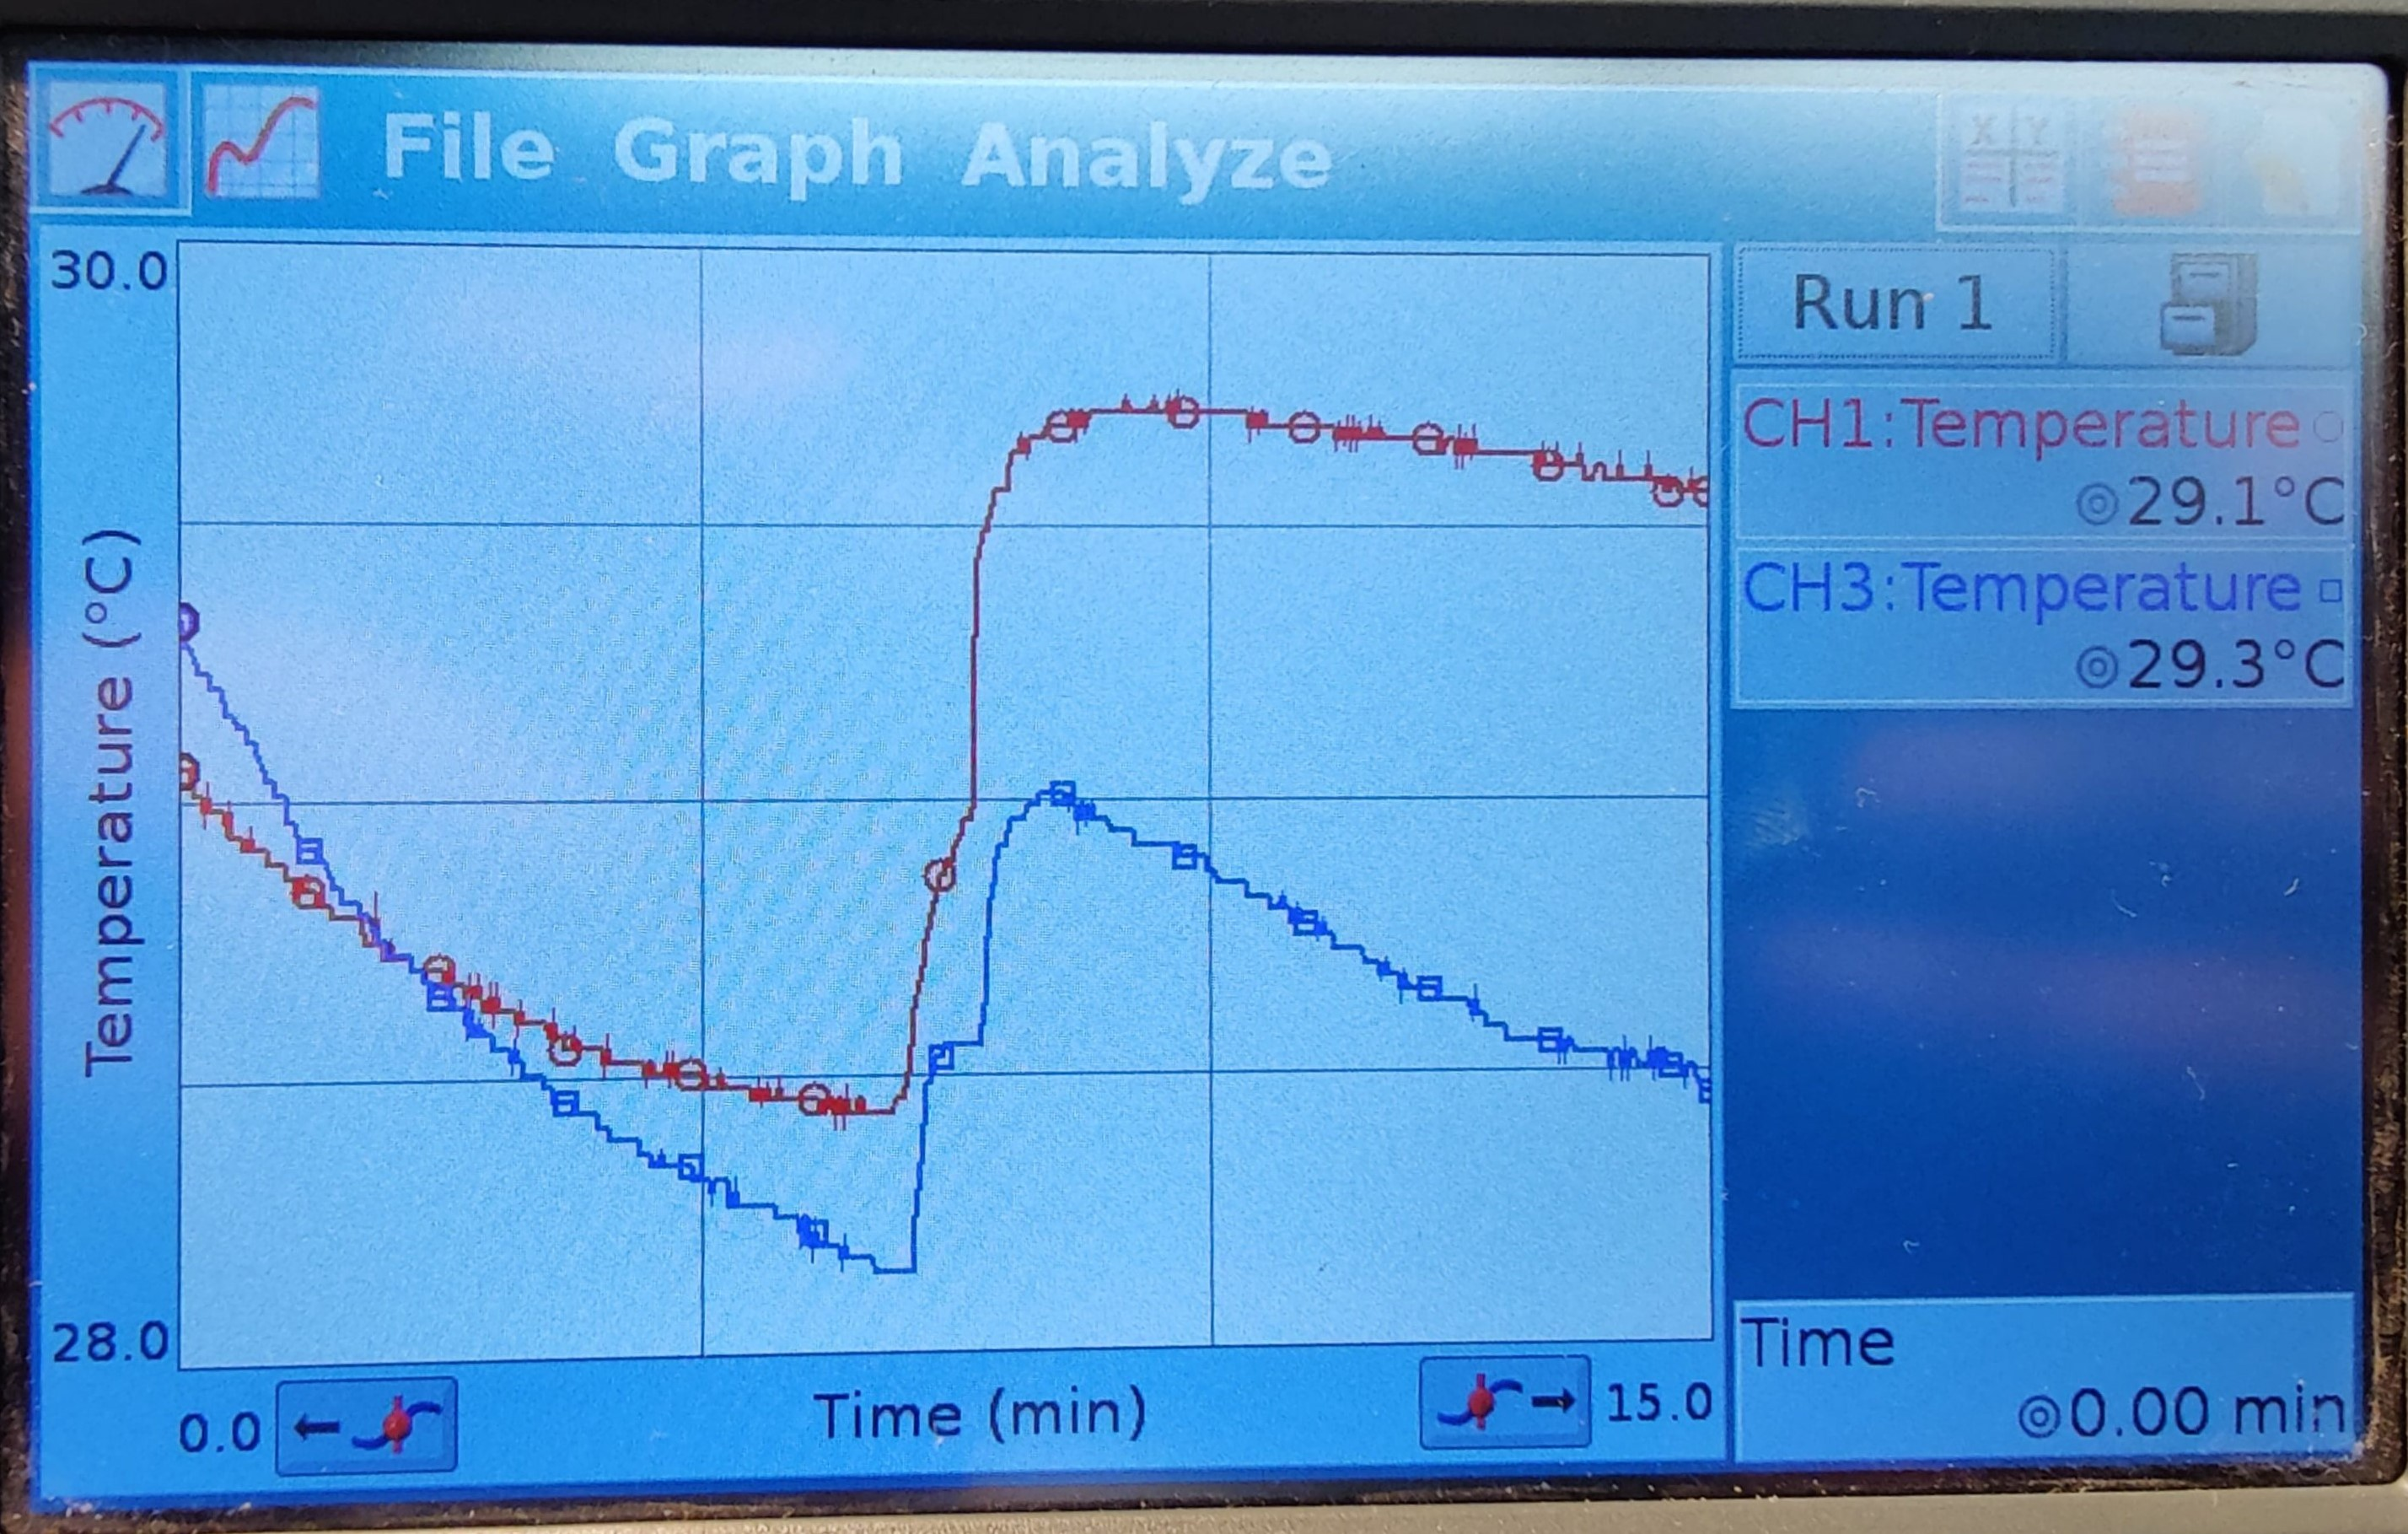
\includegraphics[width=0.4\columnwidth]{images/part1-graph.jpg}}\\
	\qquad
	\subfloat[Covered Jar]{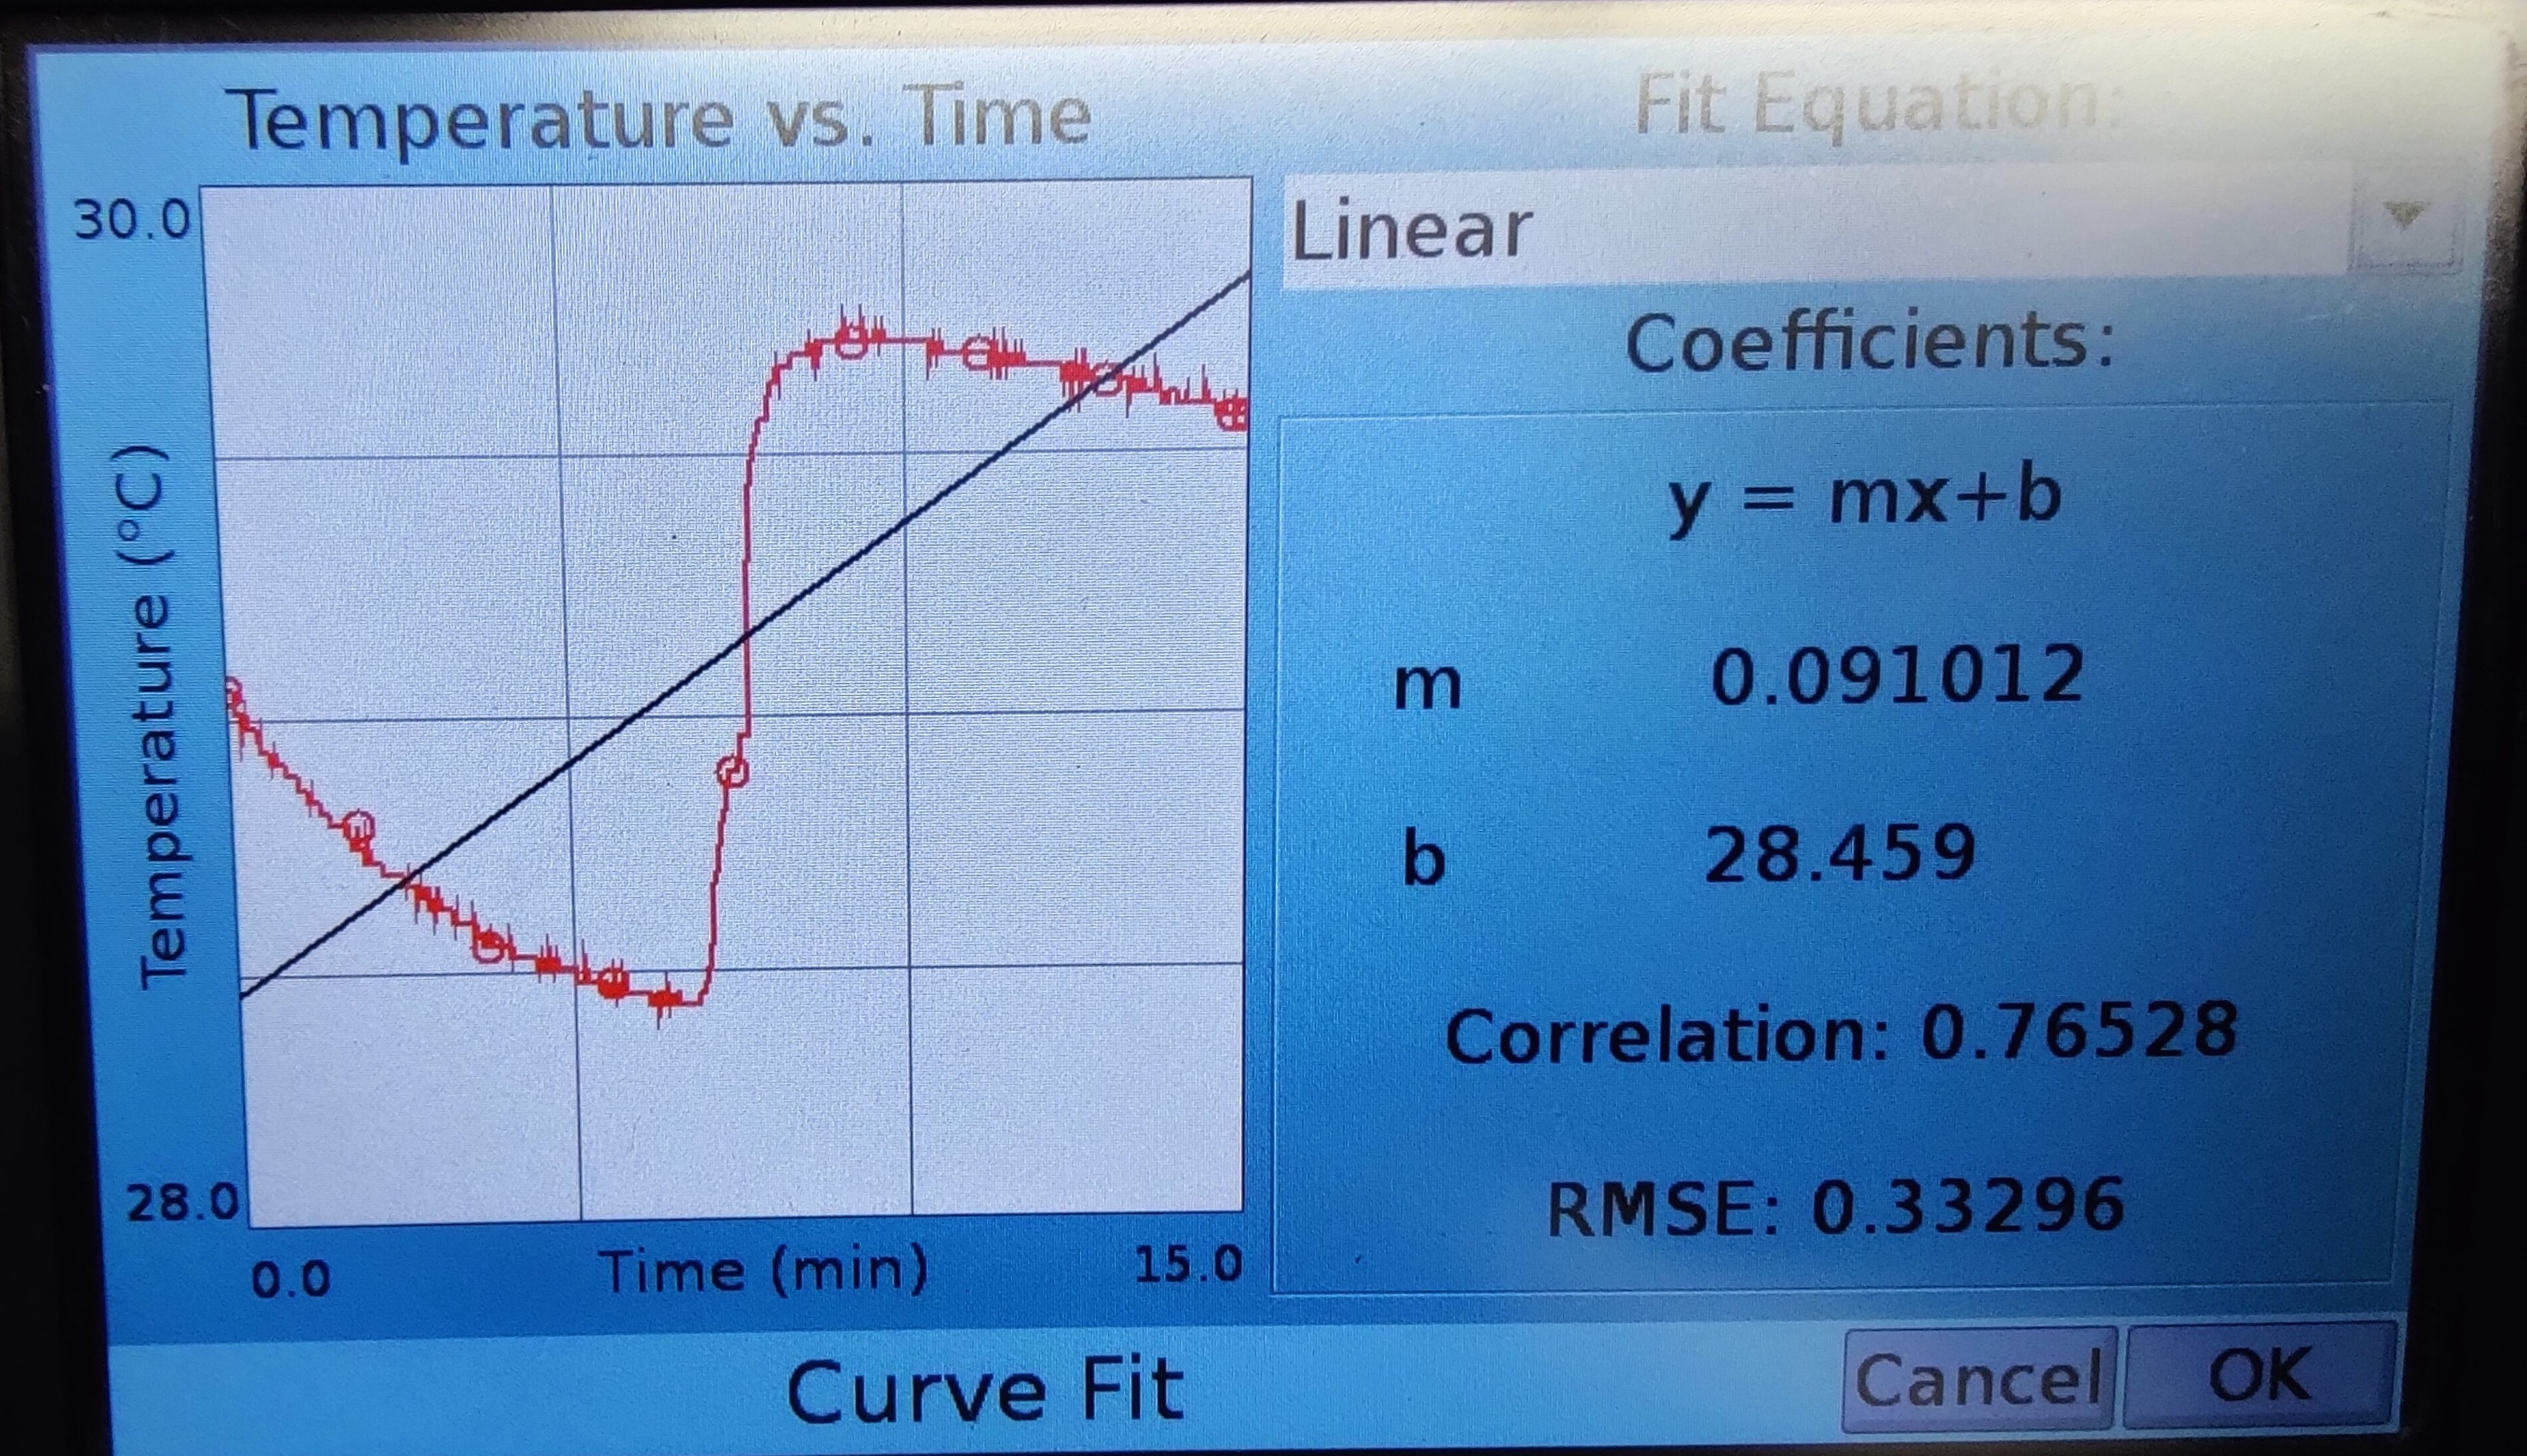
\includegraphics[width=0.4\columnwidth]{images/part1-temp1-graph.jpg}}
	\qquad
	\subfloat[Uncovered Jar]{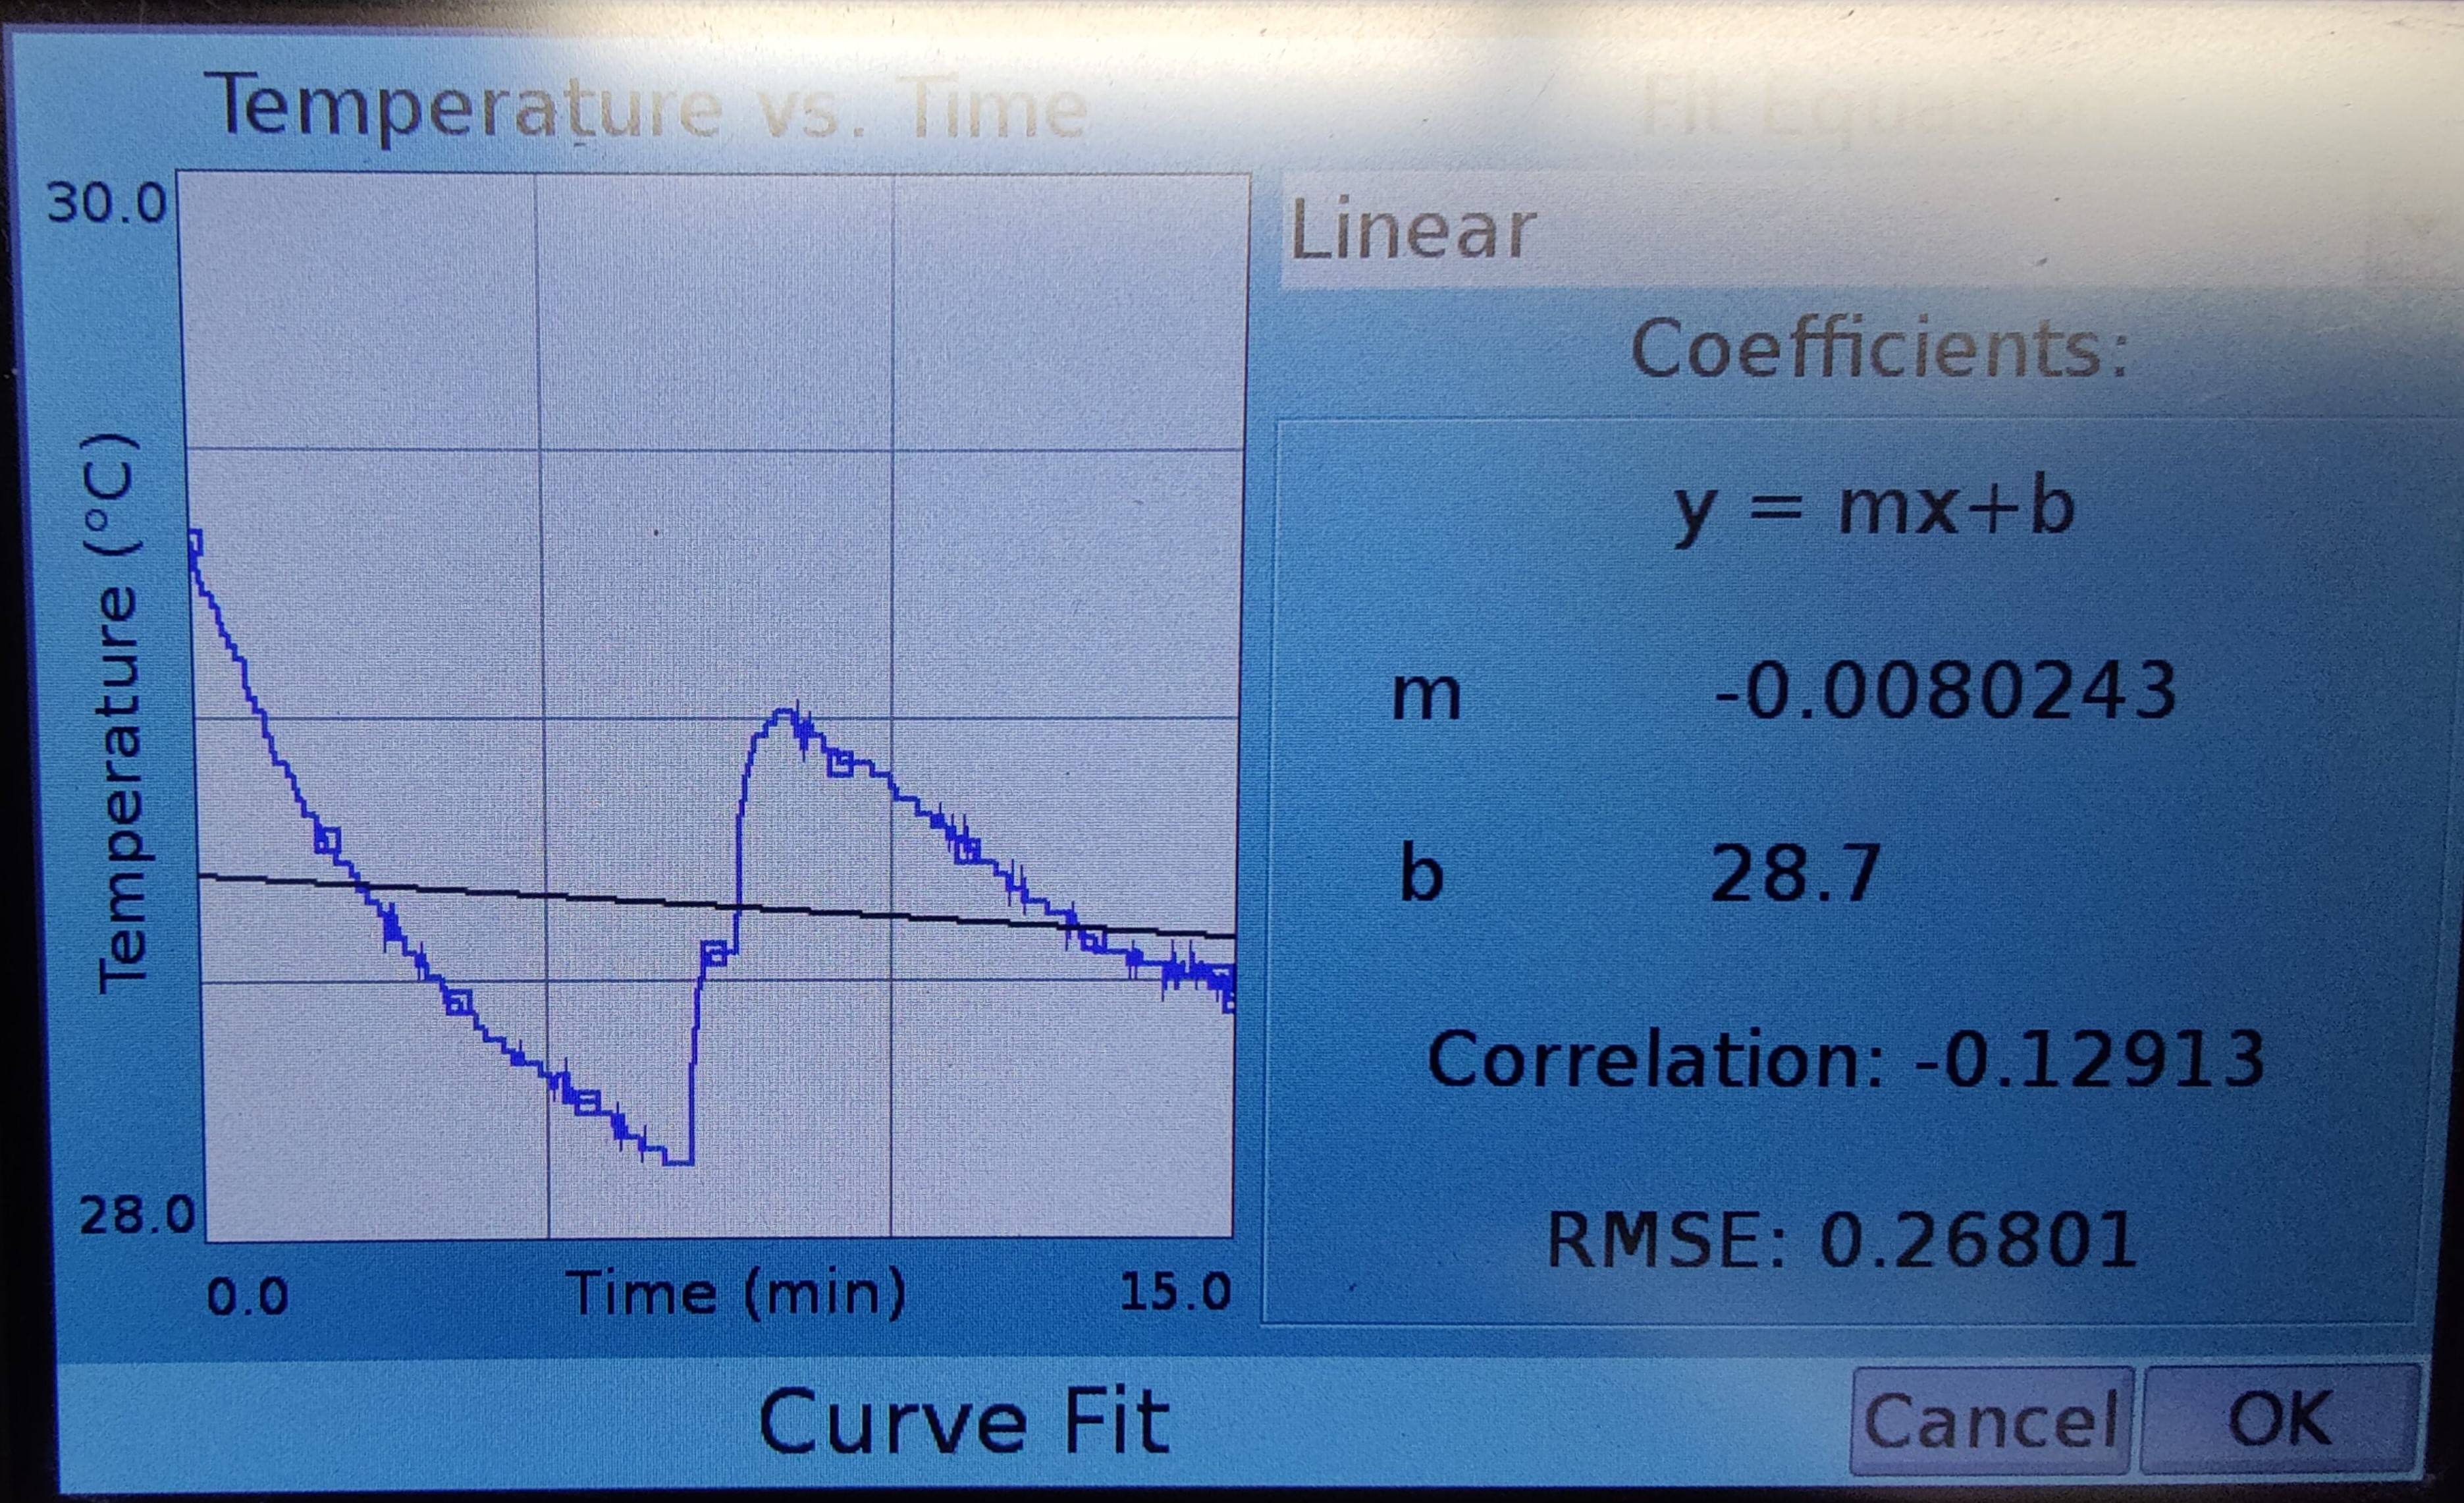
\includegraphics[width=0.4\columnwidth]{images/part1-temp2-graph.jpg}}
	\caption{Temperature Graphs}
	\label{fig:TempGraphs}
\end{figure}

\subsubsection{Temperature Table}

\begin{table}[H]
	\caption{\label{tab:Table 1} Temperature Table}
	\centering
	\begin{tabular}{c c c}
		\toprule
		                 & \textbf{Covered Jar (\degree C)}
		                 & \textbf{Uncovered Jar (\degree C)}           \\
		\cmidrule[0.4pt](r{0.125em}){1-1}%
		\cmidrule[0.4pt](lr{0.125em}){2-2}%
		\cmidrule[0.4pt](lr{0.125em}){3-3}%
		% \midrule
		\textbf{min}     & 28.4                               & 28.1    \\
		\textbf{max}     & 29.7                               & 29.3    \\
		\textbf{mean}    & 29.1                               & 28.6    \\
		\textbf{st. dev} & 0.51668                            & 0.26998
	\end{tabular}
\end{table}

\subsection{Part II: Photosynthesis and Respiration}
\subsubsection{Covered Jar}
\paragraph{O2 and CO2 Graphs}

\begin{figure}[H]
	\centering
	\subfloat[O2 and CO2]{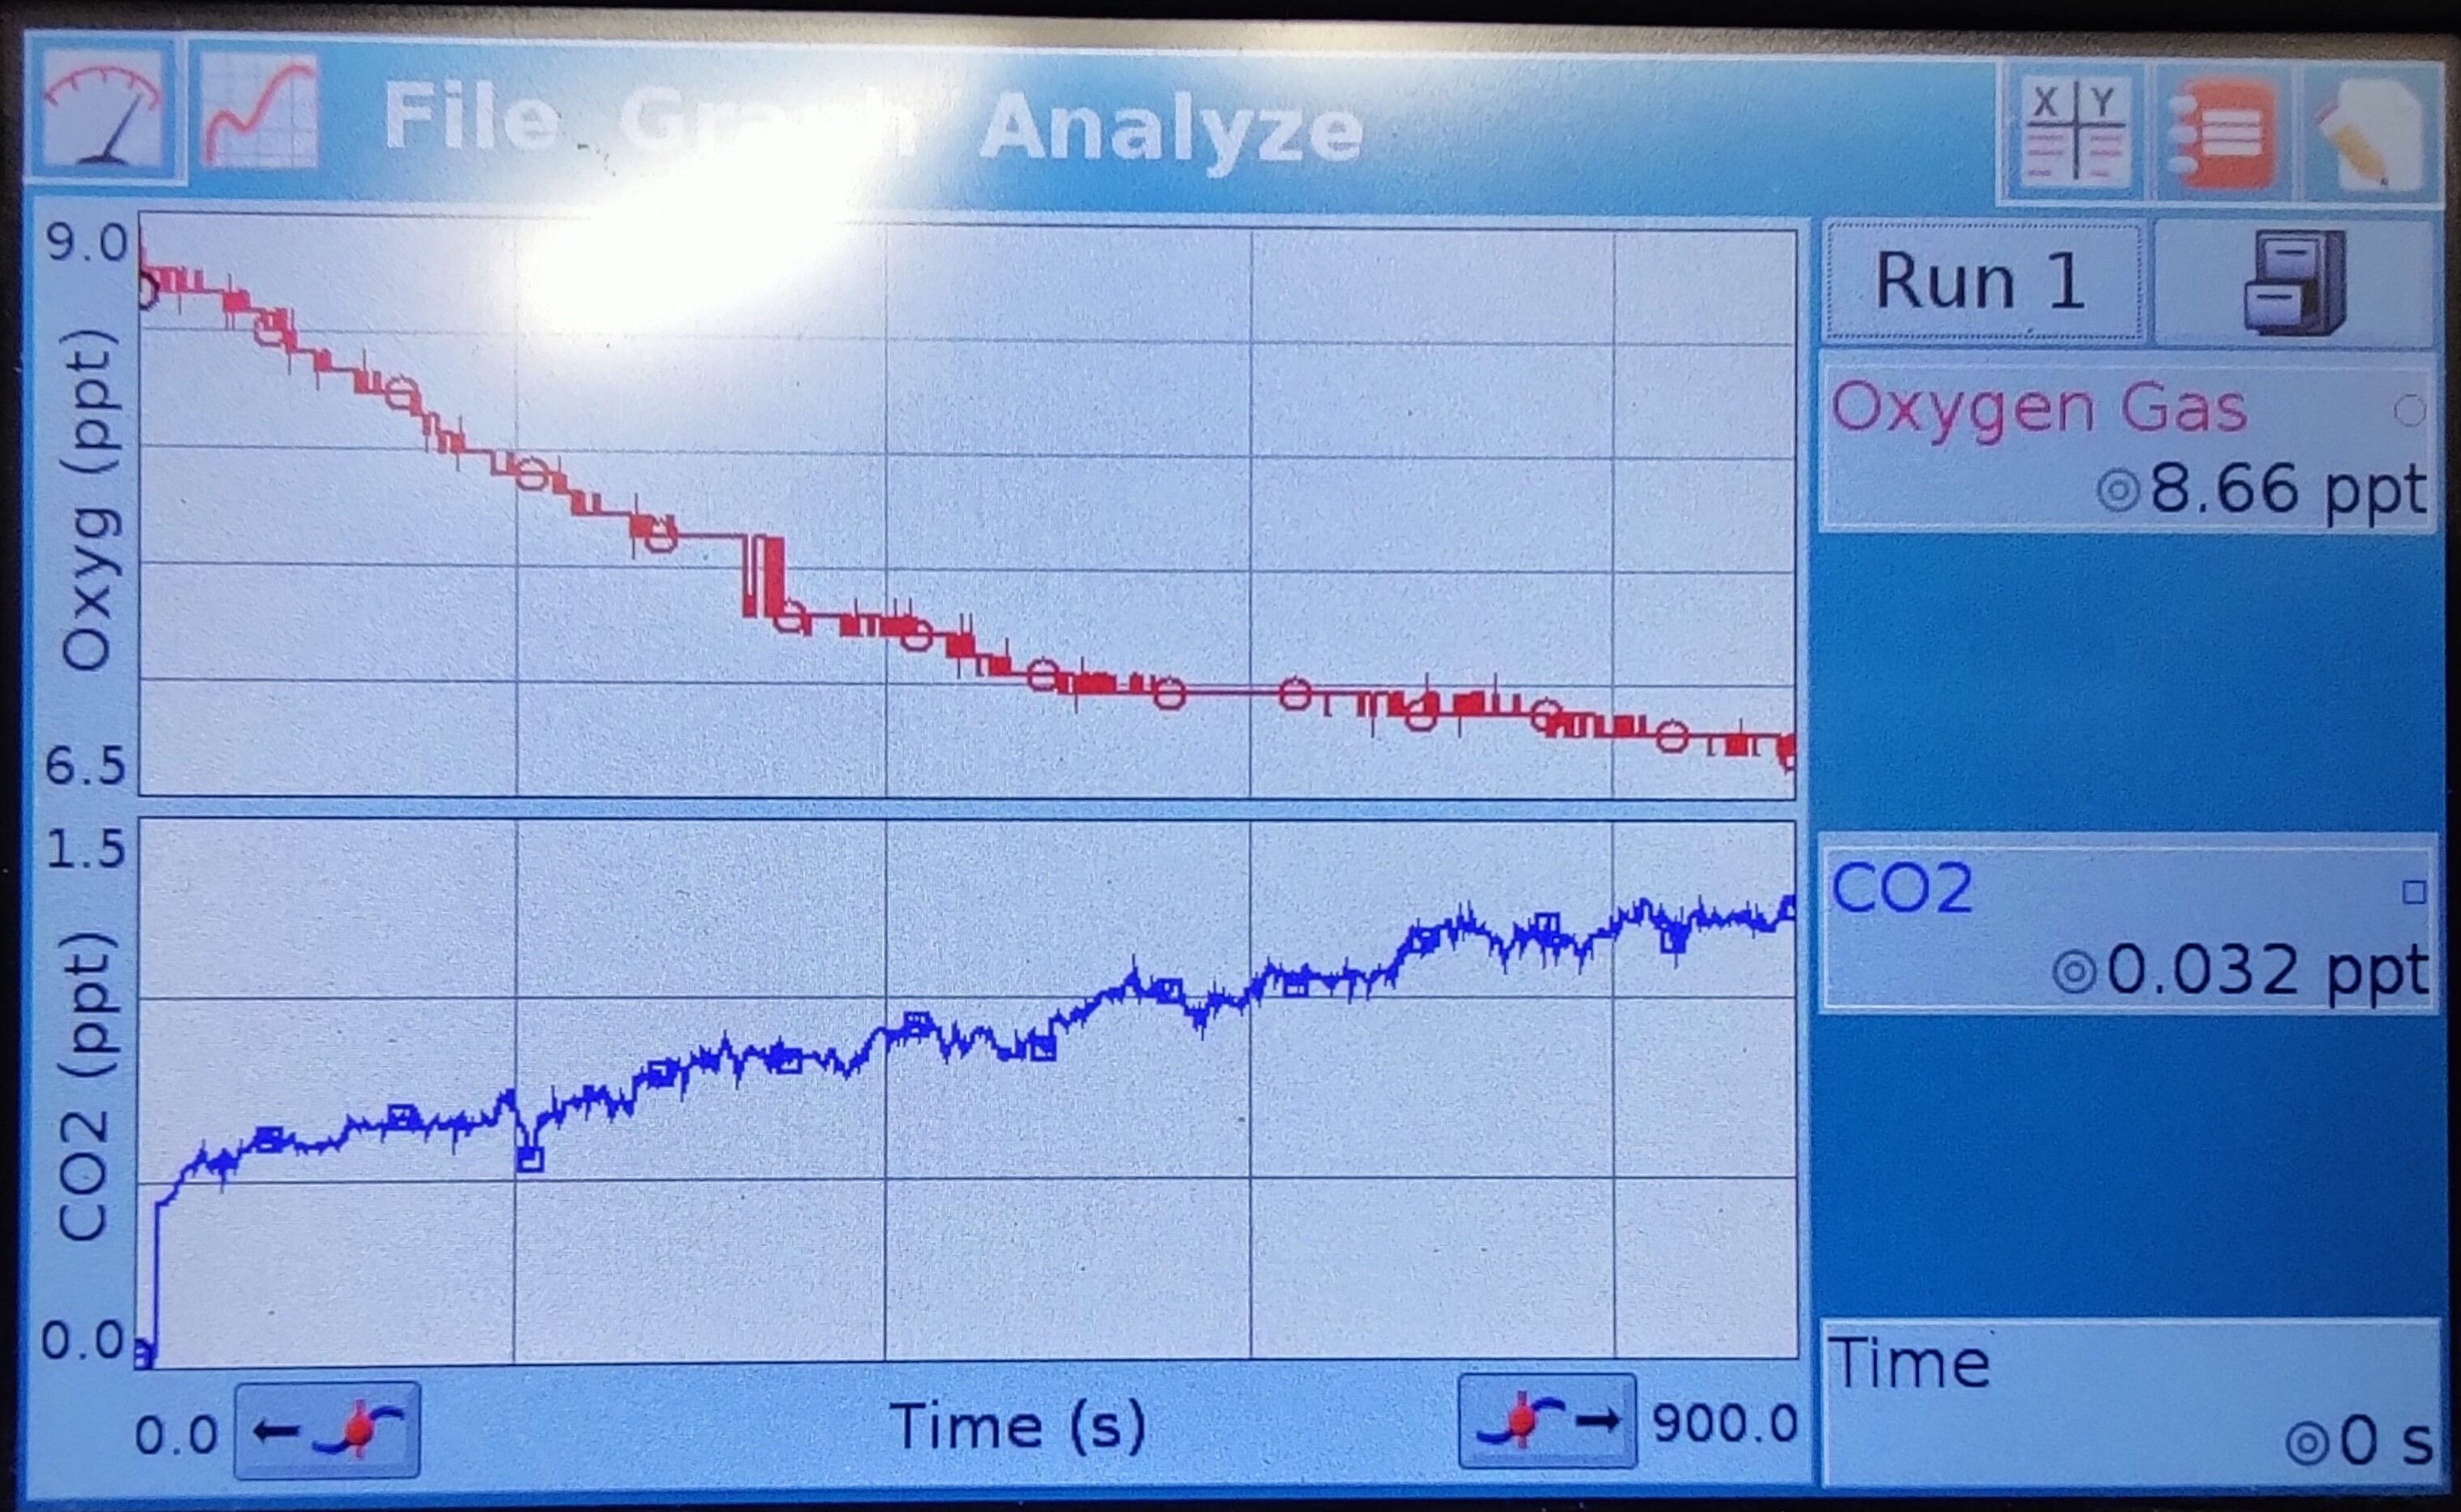
\includegraphics[width=0.4\columnwidth]{images/part2-covered-graph.jpg}}\\
	\qquad
	\subfloat[O2]{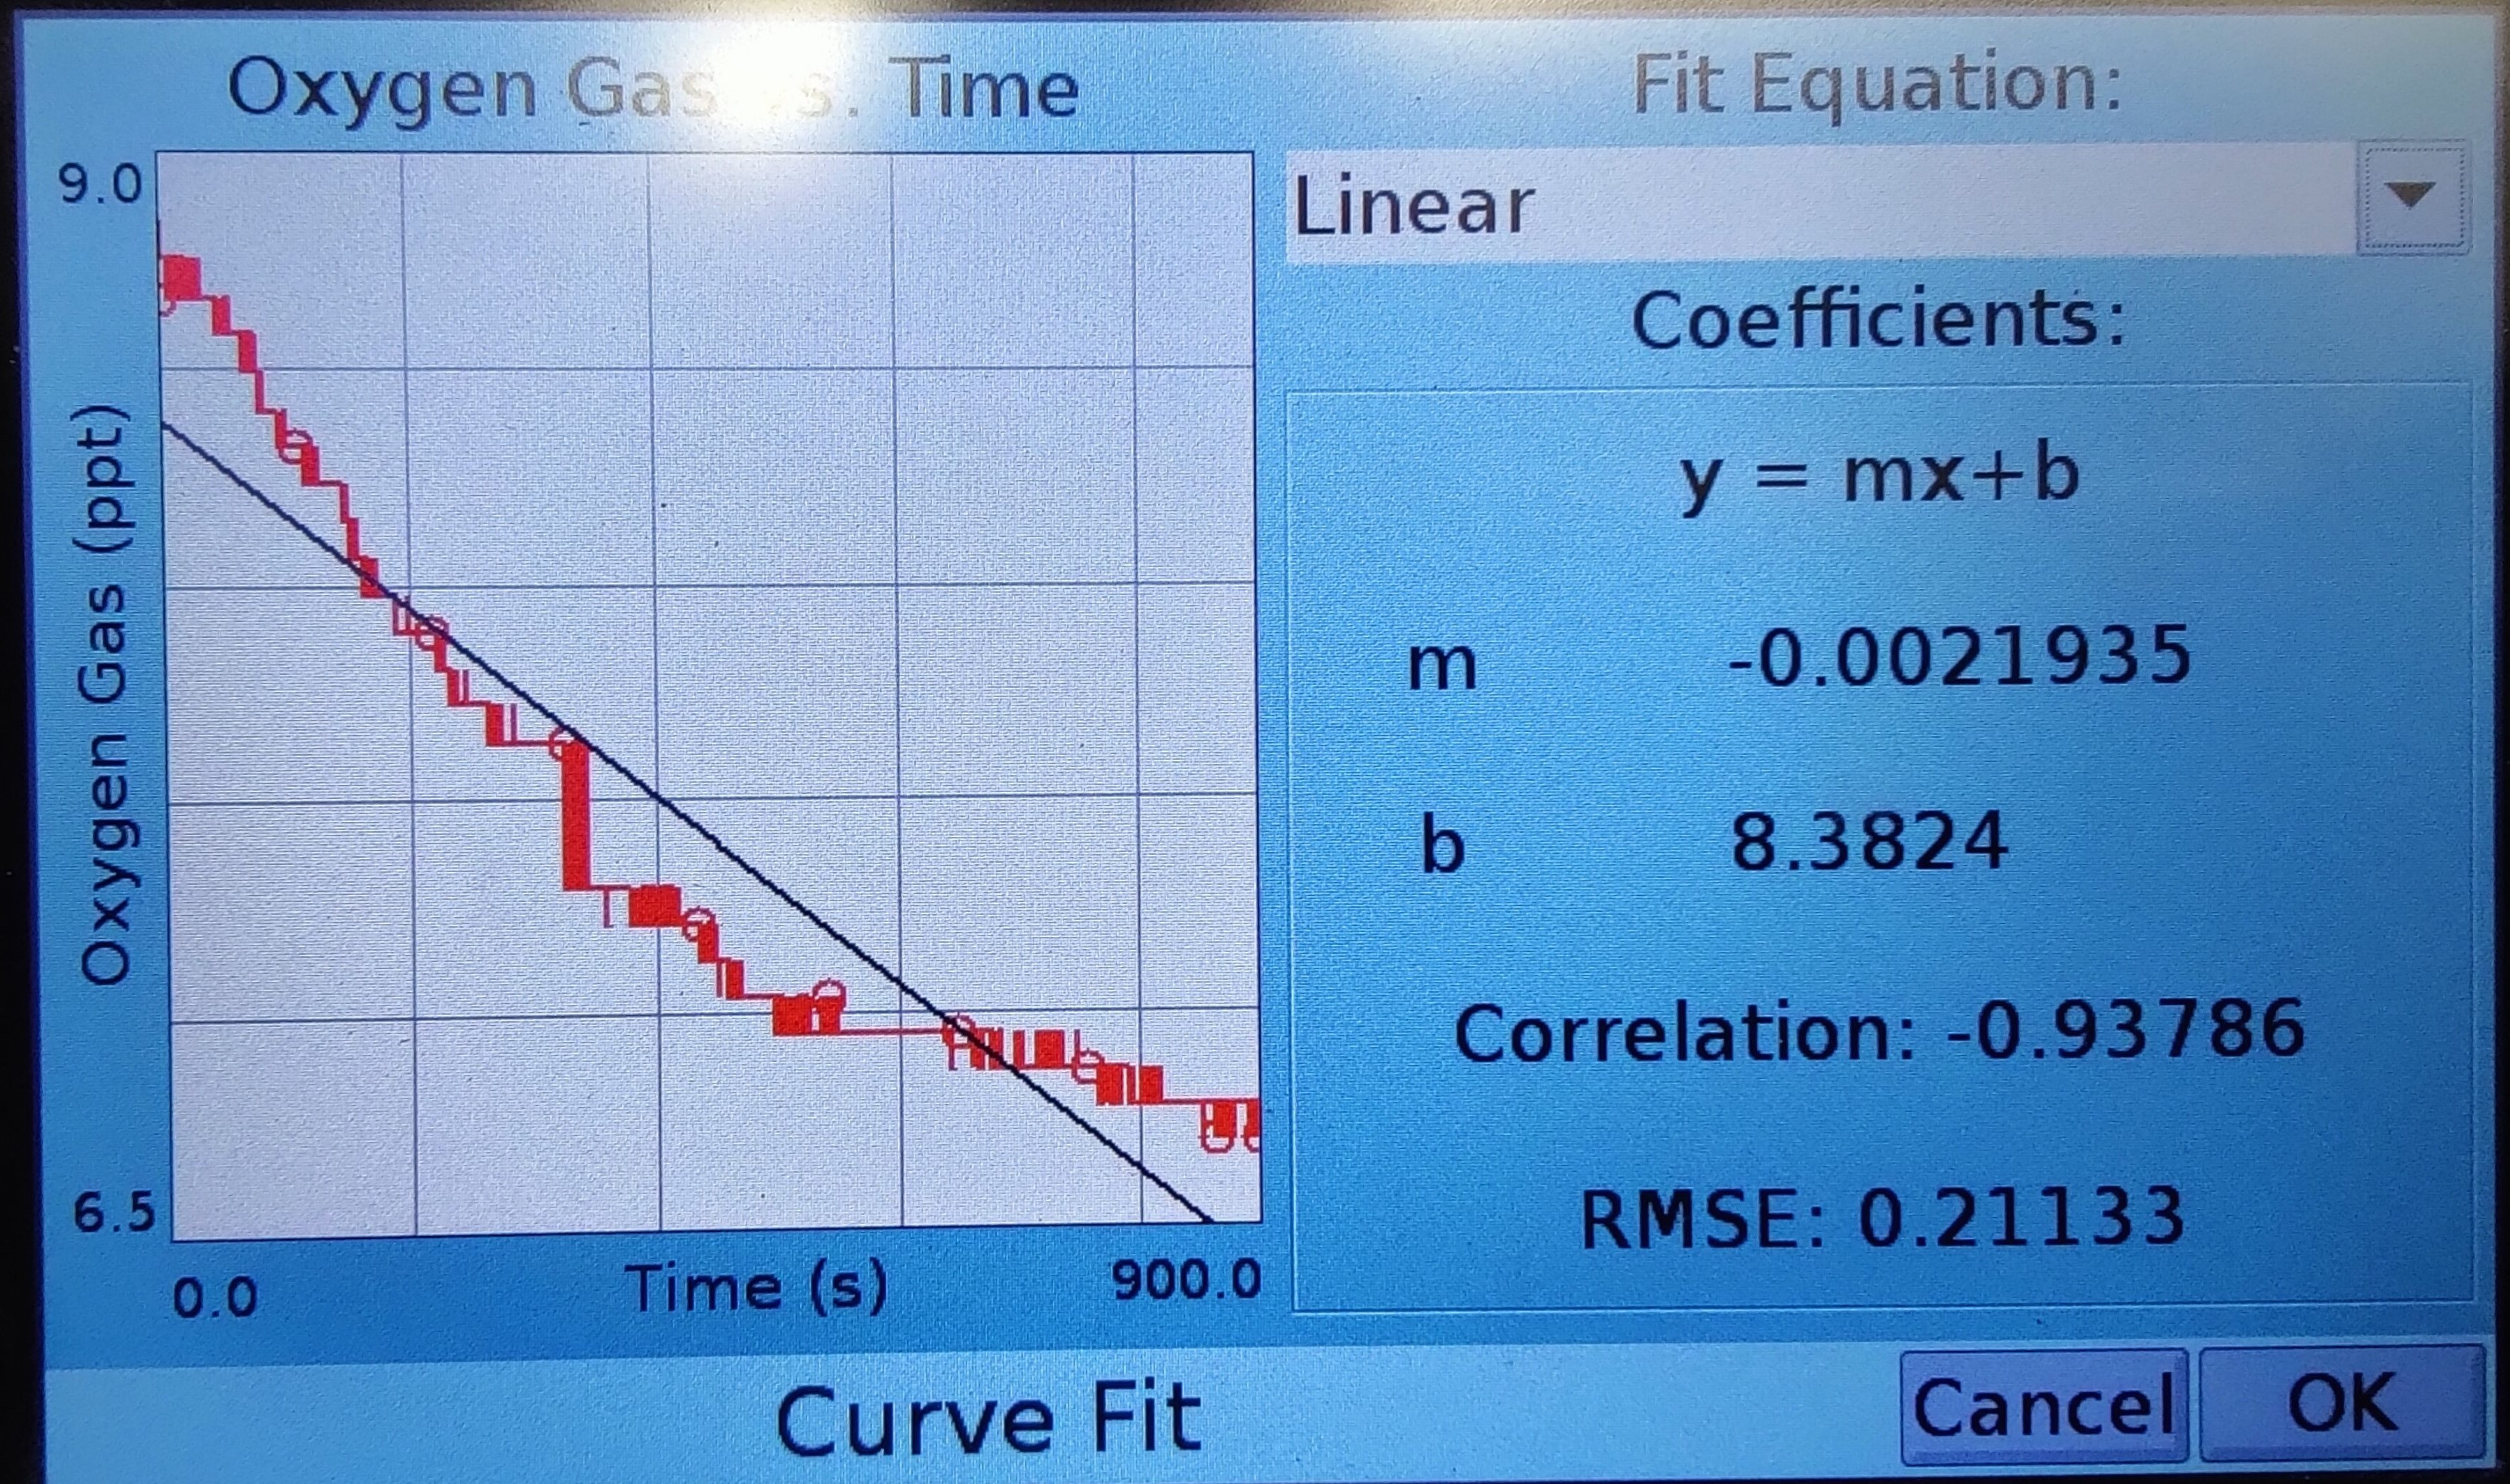
\includegraphics[width=0.4\columnwidth]{images/part2-covered-o2-graph.jpg}}
	\qquad
	\subfloat[CO2]{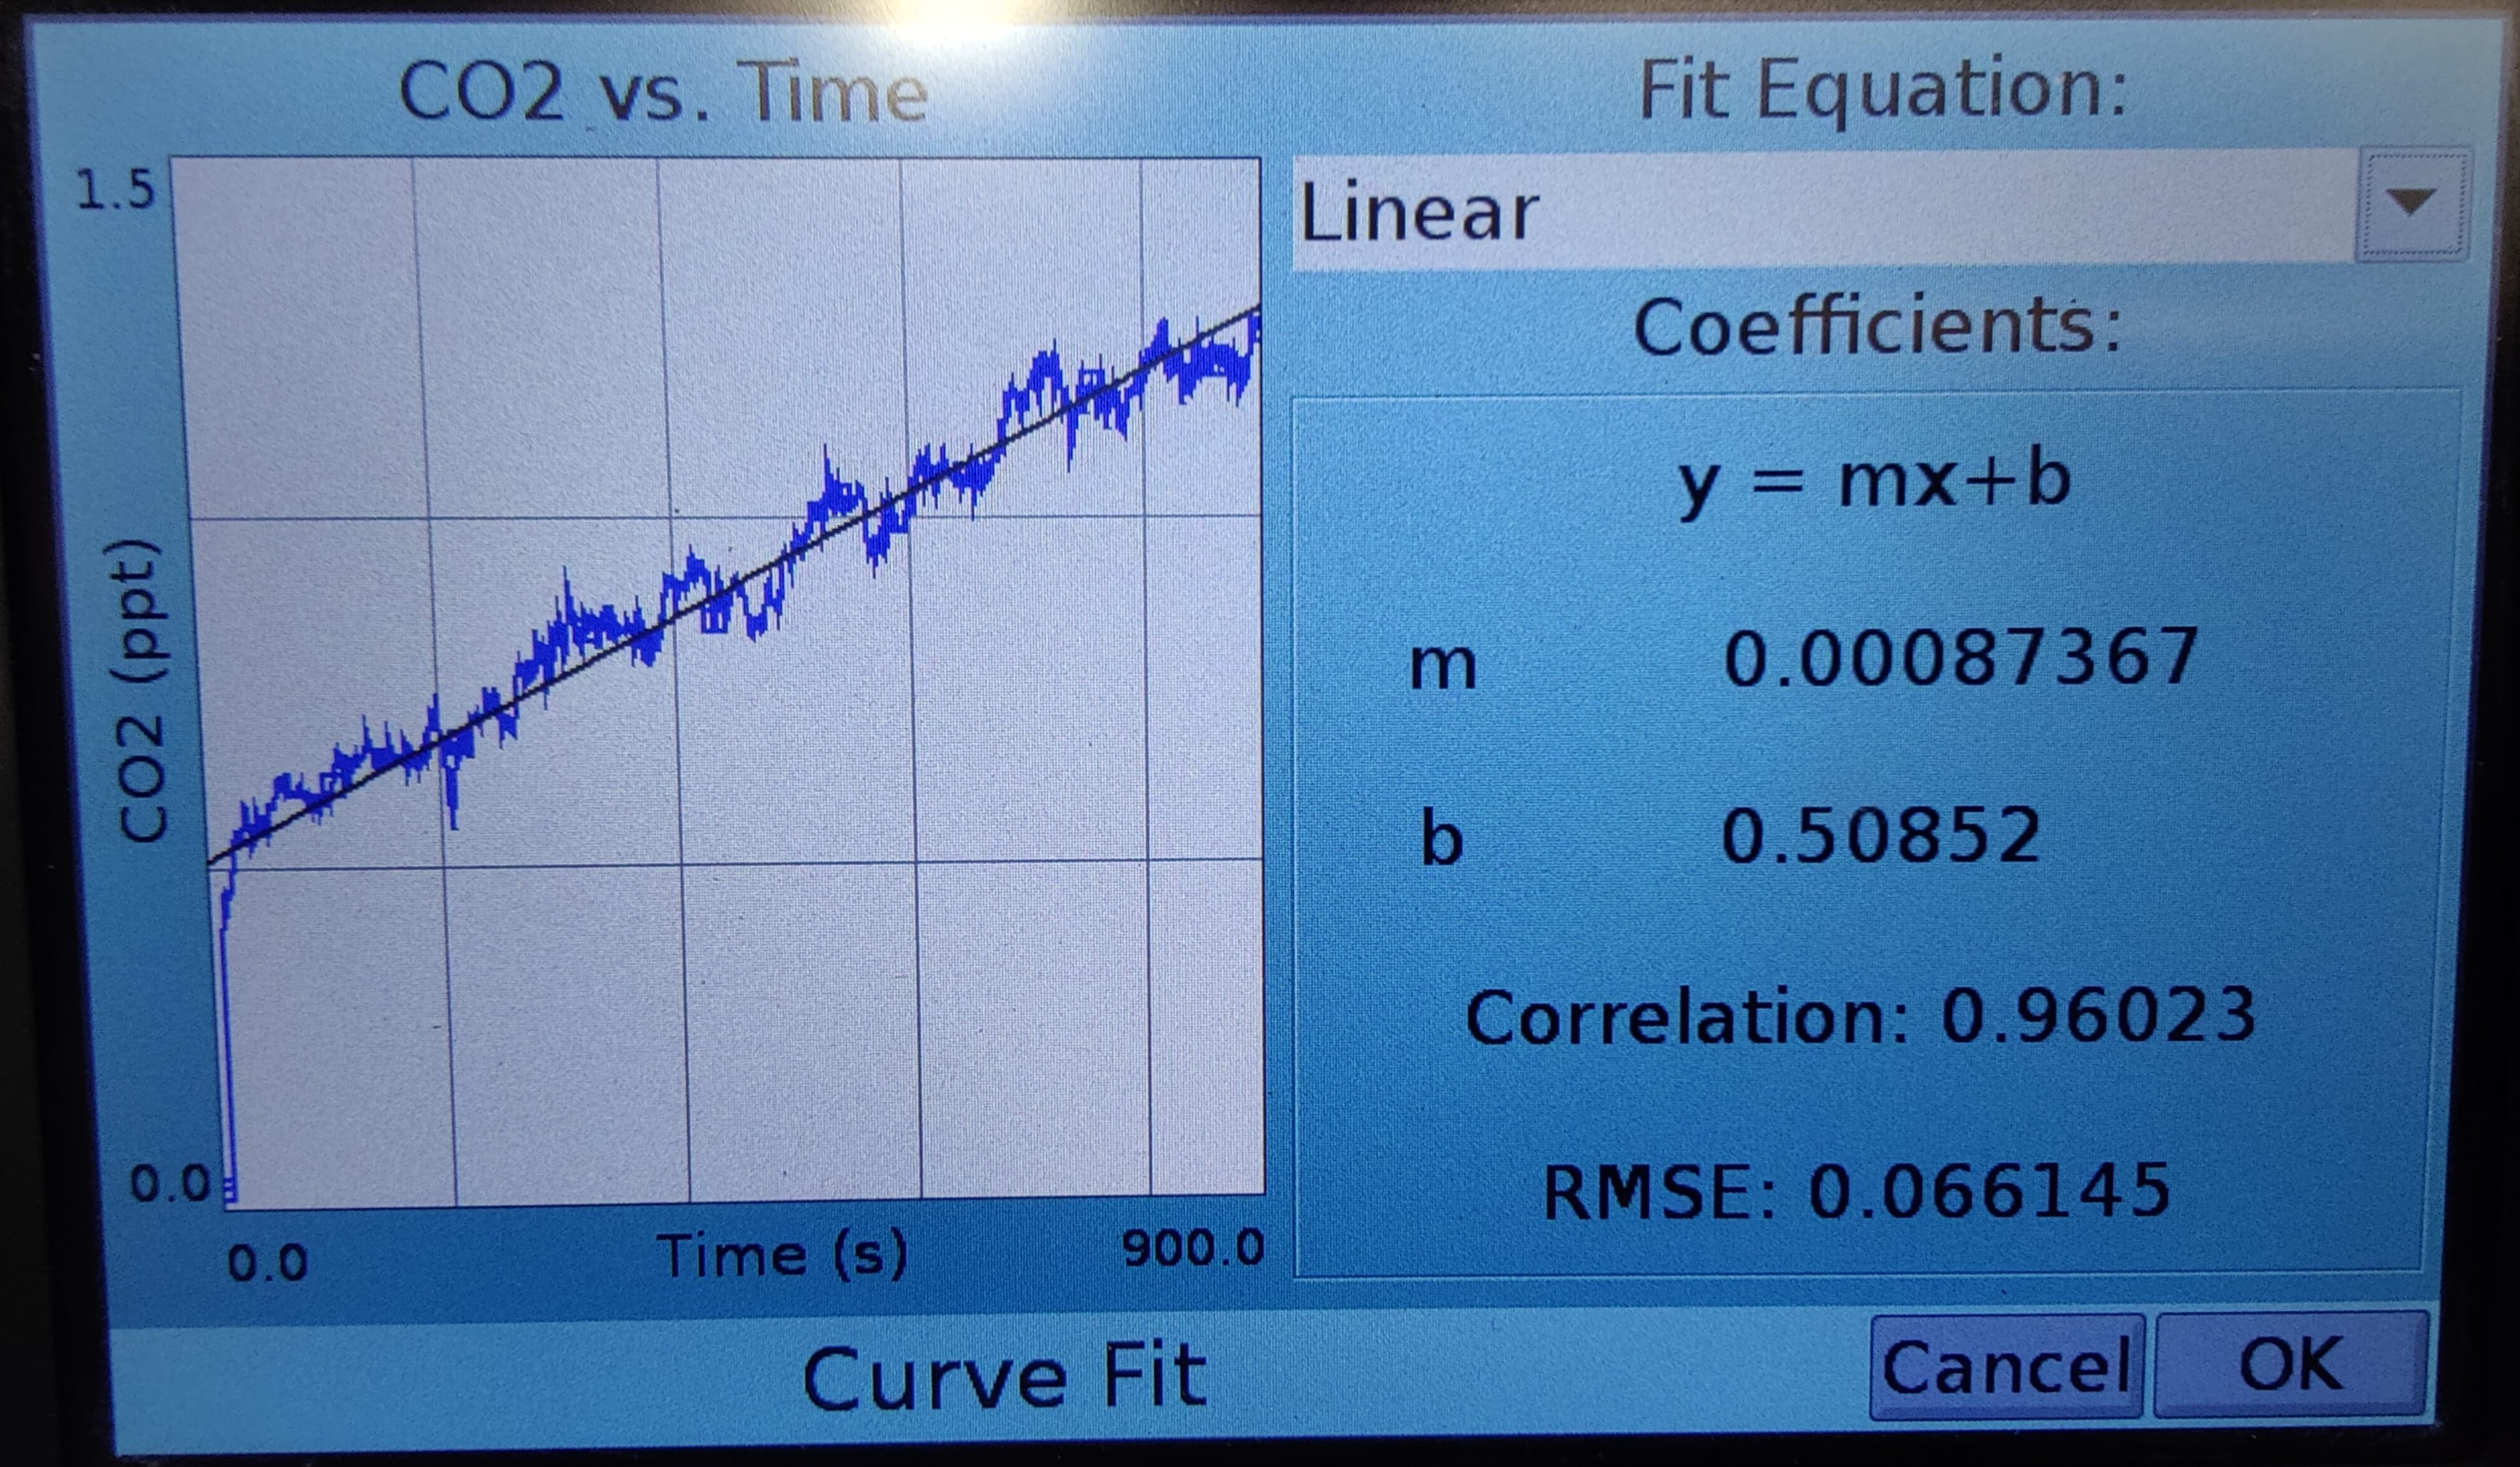
\includegraphics[width=0.4\columnwidth]{images/part2-covered-co2-graph.jpg}}
	\caption{Covered Jar}
	\label{fig:CoveredJar}
\end{figure}

\paragraph{CO2 and O2 Table}

\begin{table}[H]
	\caption{\label{tab:Table 1} O2 and CO2 Table}
	\centering
	\begin{tabular}{c c c}
		\toprule
		                 & \textbf{O2 (ppt)}
		                 & \textbf{CO2 (ppt)}           \\
		\cmidrule[0.4pt](r{0.125em}){1-1}%
		\cmidrule[0.4pt](lr{0.125em}){2-2}%
		\cmidrule[0.4pt](lr{0.125em}){3-3}%
		% \midrule
		\textbf{min}     & 6.7                & 0.032   \\
		\textbf{max}     & 8.84               & 1.277   \\
		\textbf{mean}    & 7.4                & 0.902   \\
		\textbf{st. dev} & 0.60866            & 0.23678
	\end{tabular}
\end{table}

\subsubsection{Uncovered Jar}
\paragraph{O2 and CO2 Graphs}

\begin{figure}[H]
	\centering
	\subfloat[O2 and CO2]{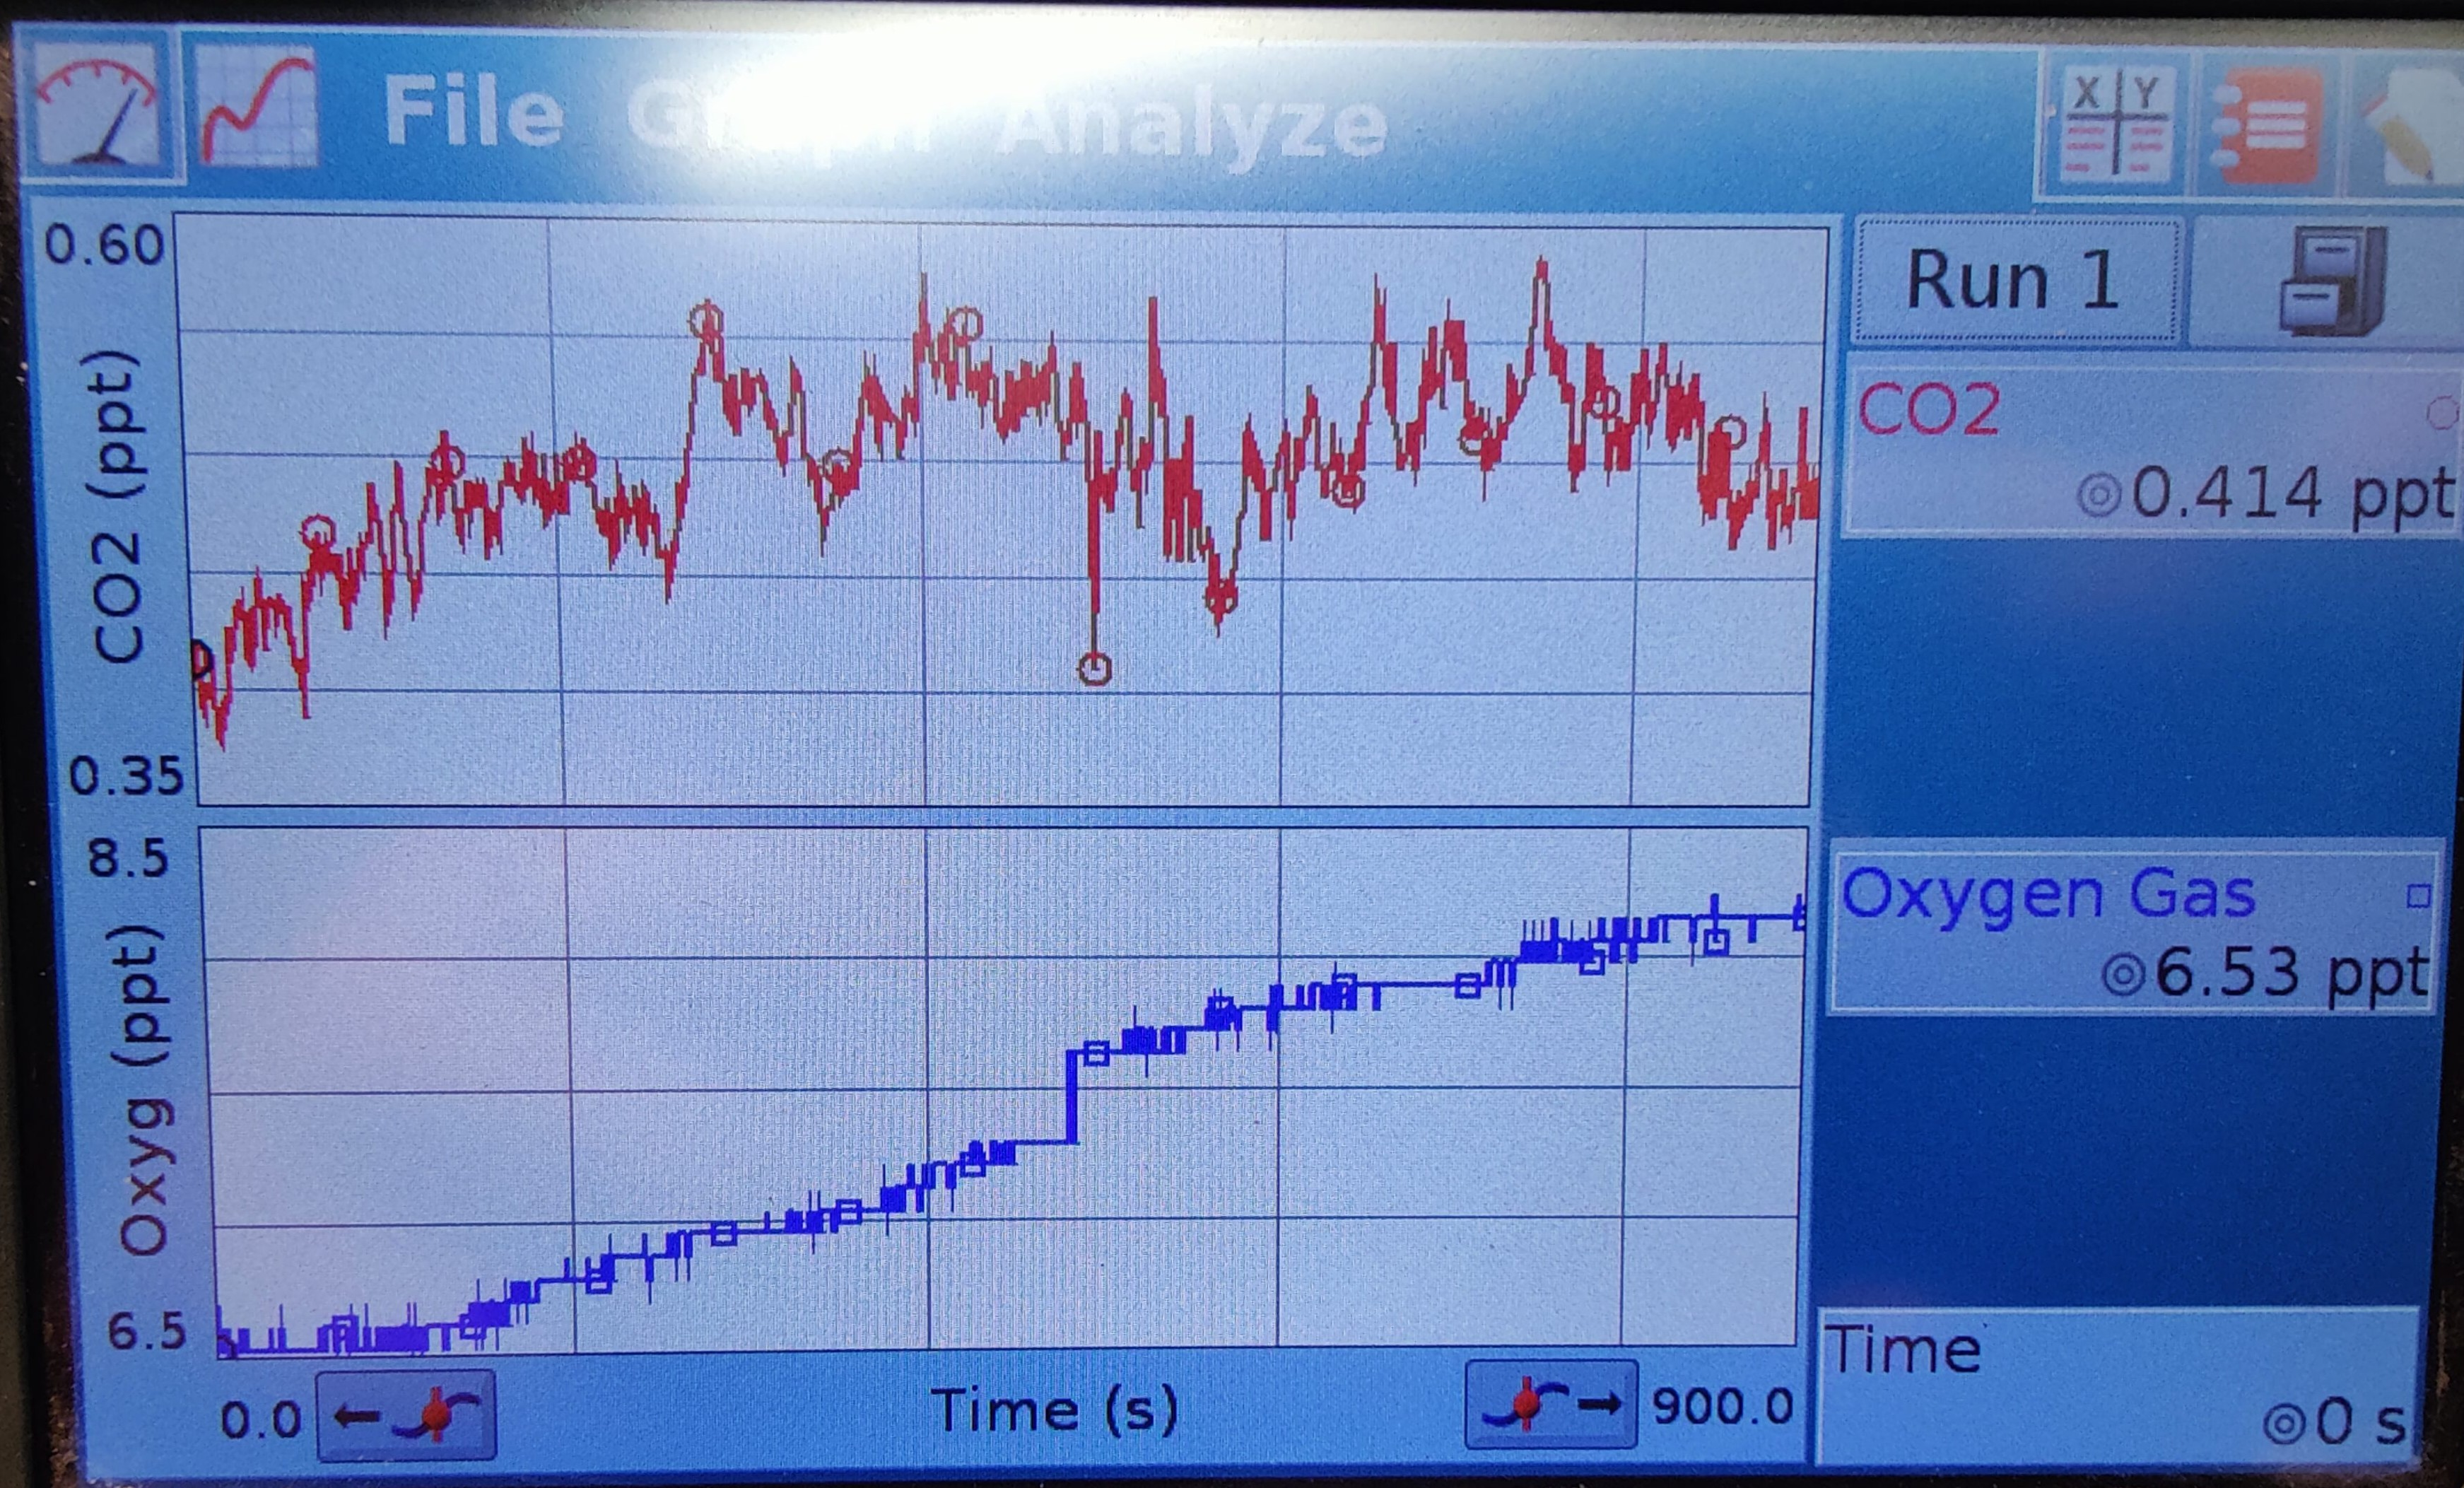
\includegraphics[width=0.4\columnwidth]{images/part2-uncovered-graph.jpg}}\\
	\qquad
	\subfloat[O2]{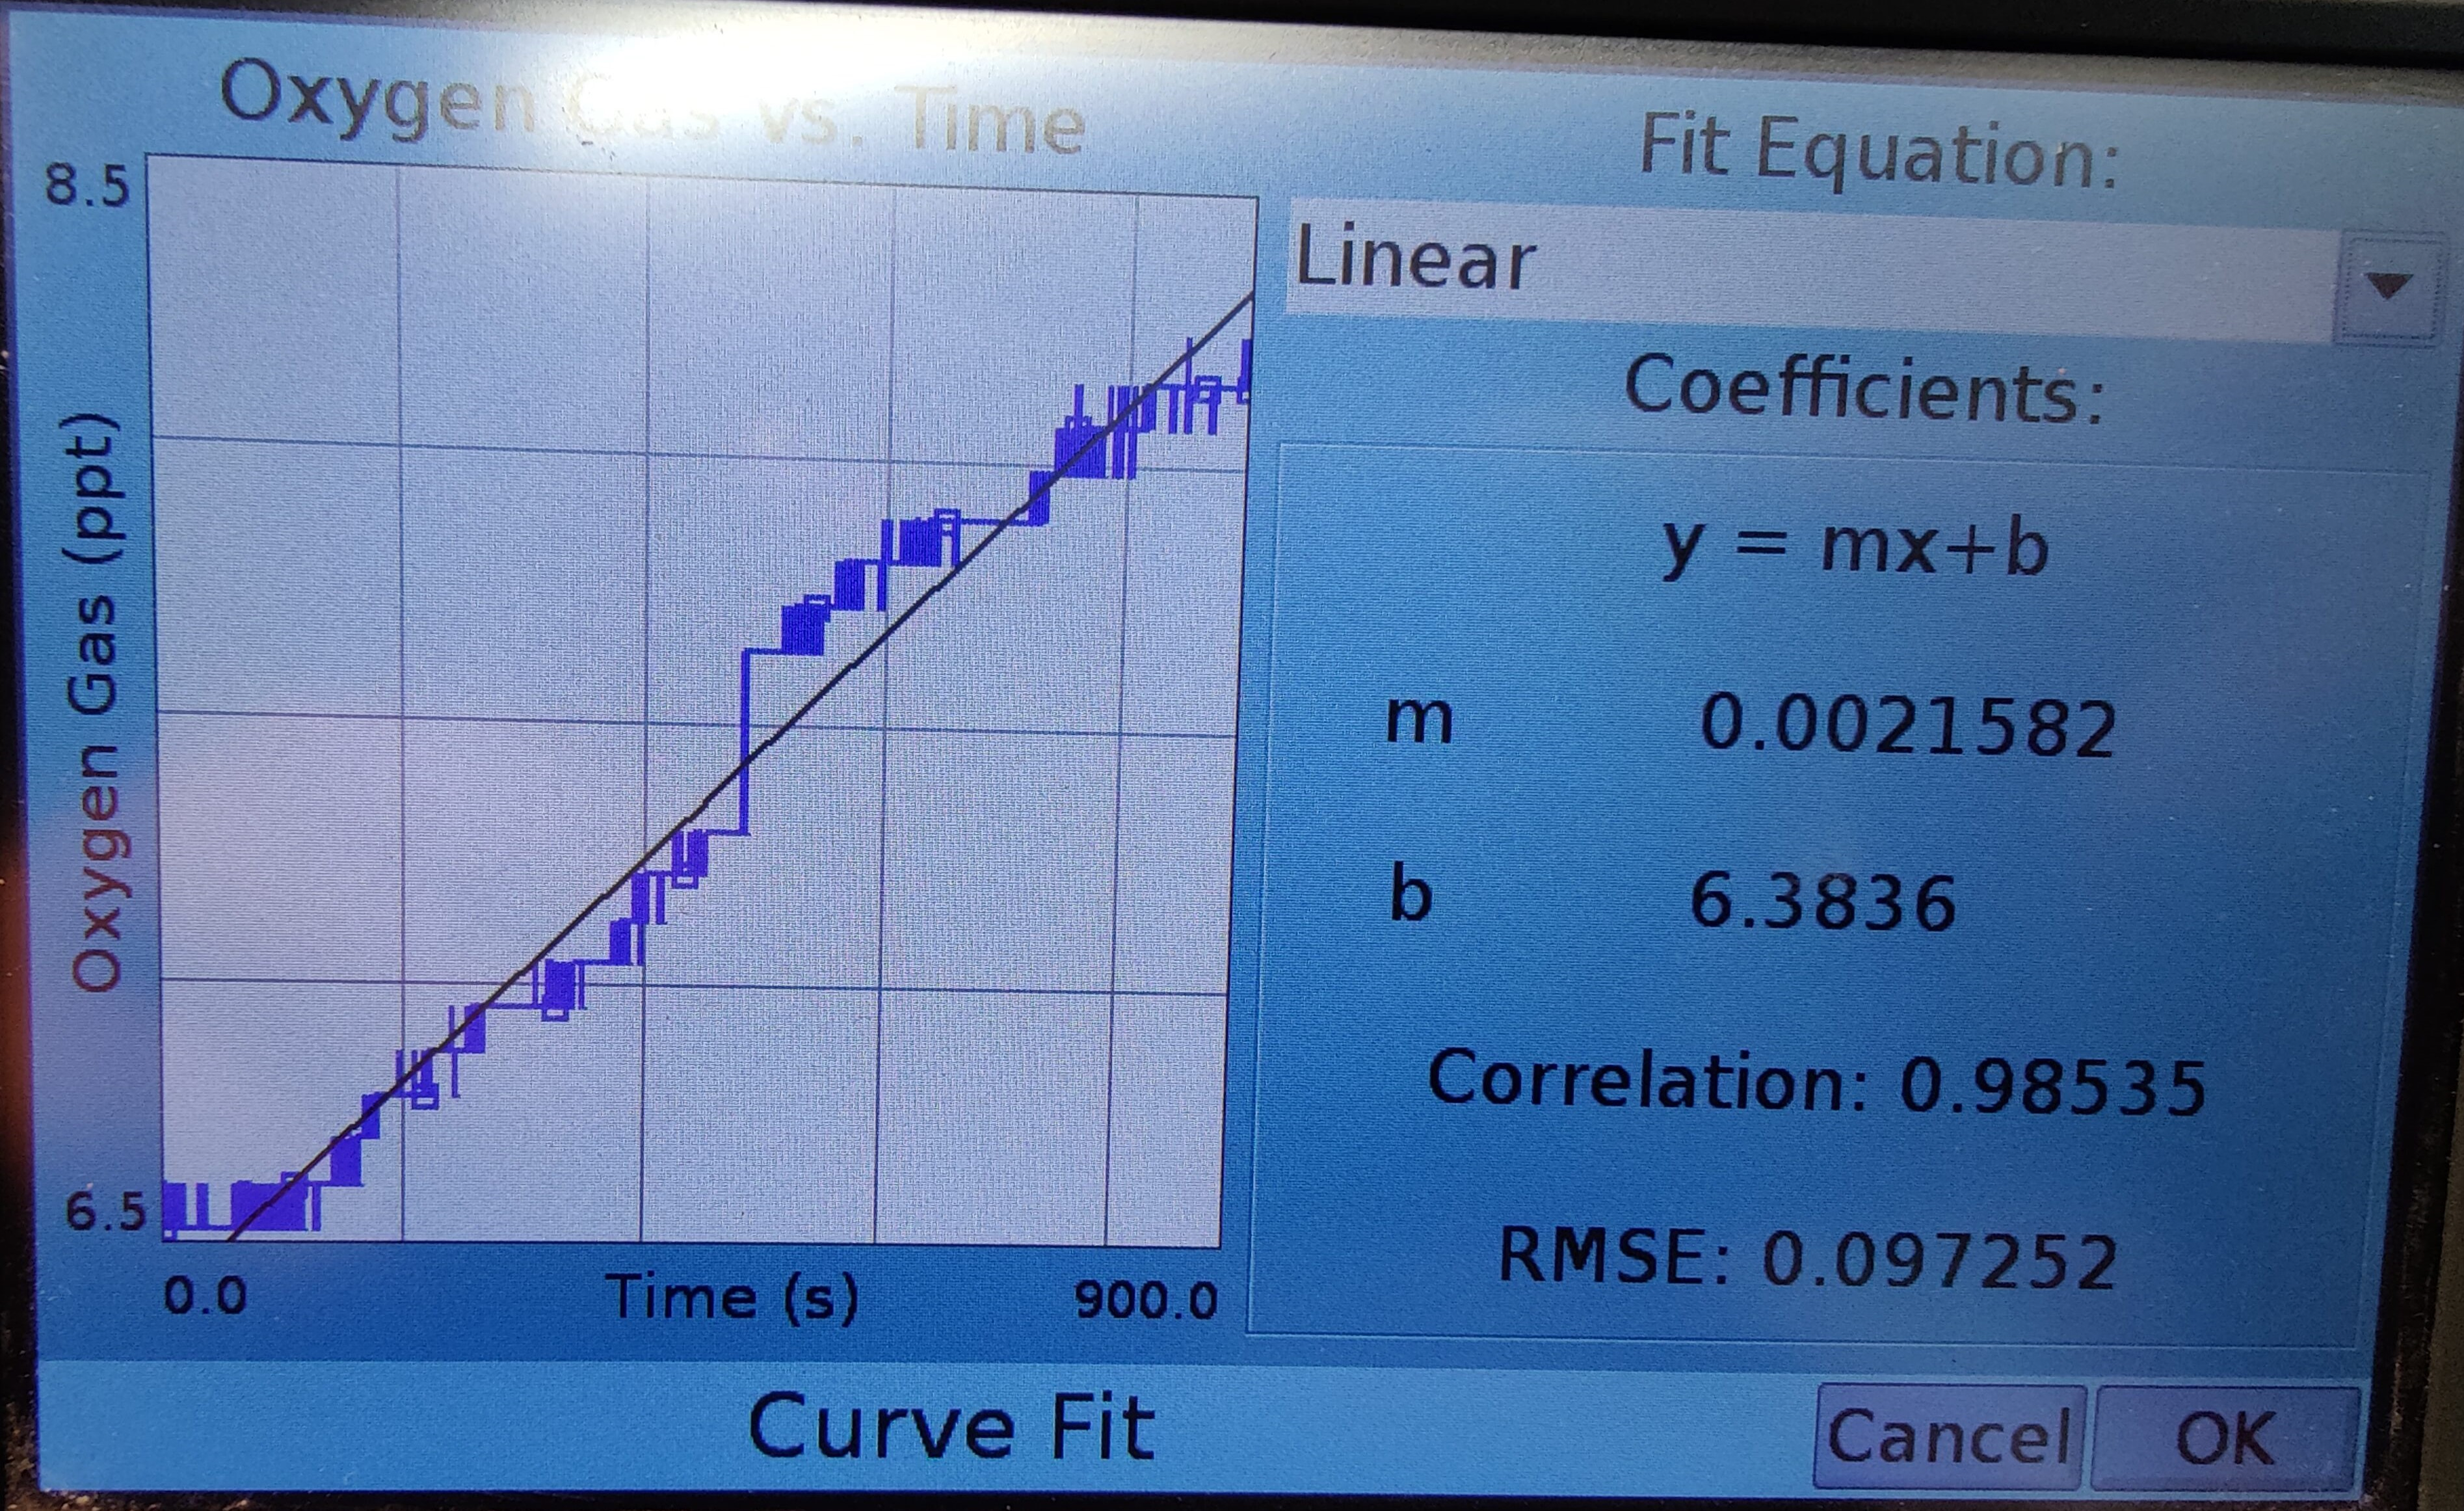
\includegraphics[width=0.4\columnwidth]{images/part2-uncovered-o2-graph.jpg}}
	\qquad
	\subfloat[CO2]{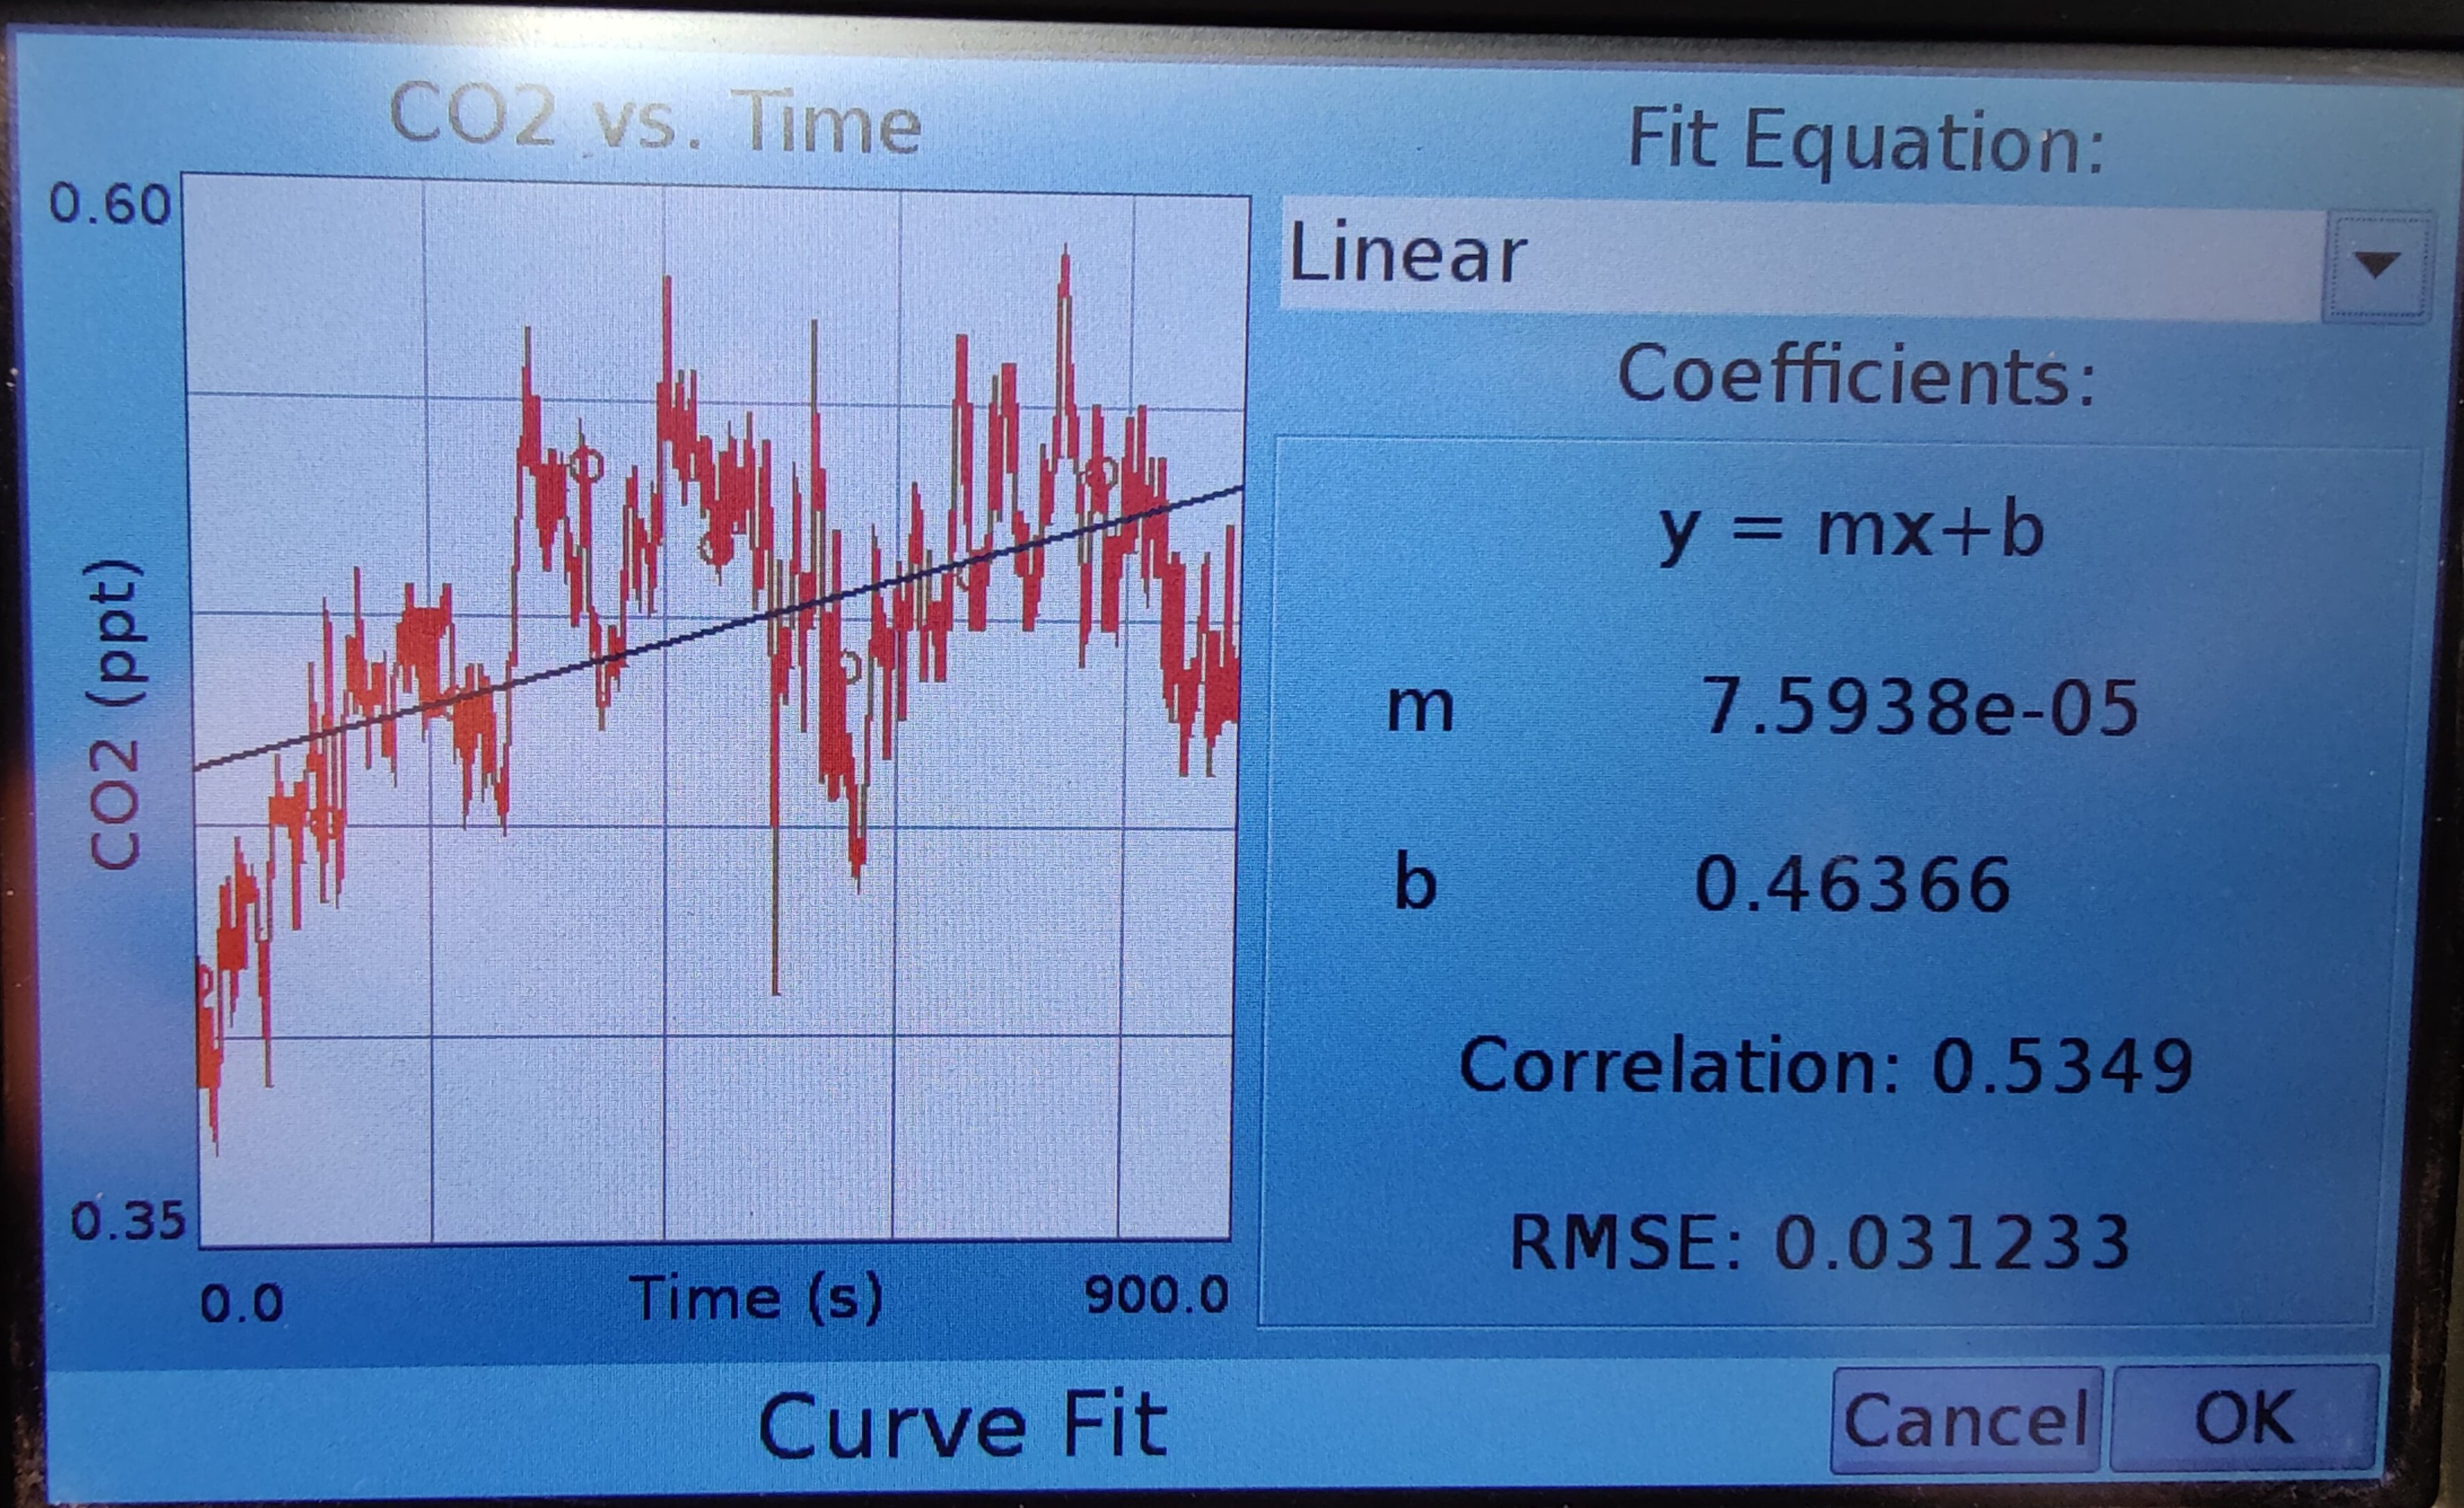
\includegraphics[width=0.4\columnwidth]{images/part2-uncovered-co2-graph.jpg}}
	\caption{Uncovered Jar}
	\label{fig:UncoveredJar}
\end{figure}

\paragraph{CO2 and O2 Table}

\begin{table}[H]
	\caption{\label{tab:Table 1} O2 and CO2 Table}
	\centering
	\begin{tabular}{c c c}
		\toprule
		                 & \textbf{O2 (ppt)}
		                 & \textbf{CO2 (ppt)}           \\
		\cmidrule[0.4pt](r{0.125em}){1-1}%
		\cmidrule[0.4pt](lr{0.125em}){2-2}%
		\cmidrule[0.4pt](lr{0.125em}){3-3}%
		% \midrule
		\textbf{min}     & 6.53                & 0.376   \\
		\textbf{max}     & 8.24               & 0.586   \\
		\textbf{mean}    & 7.35               & 0.498   \\
		\textbf{st. dev} & 0.56999            & 0.036946
	\end{tabular}
\end{table}

\section{Conclusion}
For part A of the experiment, we observed that the covered jar had a higher
temperature than the uncovered jar. This is because the covered jar was
insulated, and the heat was trapped inside. This is similar to the greenhouse
effect, where the heat is trapped inside the earth's atmosphere.

For part B of the experiment, we observed that the covered jar had a higher
concentration of CO2 and a lower concentration of O2 than the uncovered jar.
This is because the plant inside the uncovered jar was photosynthesizing, and
releasing O2 and absorbing CO2. The plant inside the covered jar was
respiring, and releasing CO2 and absorbing O2.

\section{Questions To Ponder}
\subsection{Part A:}

\begin{enumerate}
    \item Explain with reasons which beaker covered or uncovered has the greatest temperature change?
    
	The covered beaker has the greatest temperature change because it replicates the greenhouse effect, similar to 
	the greenhouse gases present in our atmosphere, so the greenhouse effect is more prominent in the covered beaker. Due 
	to which it a greater temperature change compared to the uncovered beaker, this is because the plastic wrap traps 
	heat within ther beaker leading to a rise in temperature significantlty higher than the uncovered beaker.
    \item Which beaker has the greatest rate of temperature change and why?
    
	The  uncovered beaker has the greatest rate of temperature change, as it not covered by plastic wrap, i.e. less insulation
	heat transfers more easily between inside of beaker and surrounding environment. This leads to heat escaping 
	and thus a greater rate of temperature change.
    \item What is slope and the rate of reaction?
    
    In a graph the slope is of the curve at any given point and this slope represents the rate
	of reaction. The steeper the slope, faster the reaction. Similarly the rate of reaction
	is a measure of how fast a reaction occurs. The rate of reaction is the change in concentration of produts or reactants.	
	\item Why might the greenhouse effect be a problem for our earth?
	
	The greenhouse might be a problem for our earth because it traps heat within our atmosphere and this is 
	intensified by human acitivies such as burning fossil fuels, leading to a rise in temperature, and 
	hence numerous problems arise. For example, global qarming, leads to melting of ice caps, which fruther leads to
	rise in sea level, and due to all of this many coastal areas will be submerged, and many more to come.
    \item Did the model greenhouse warm faster or slower than the control? What do you think caused the difference?
    The model greenhouse warmed faster than the control, this is because the plastic wrap has insulating proerties 
	and traps heat within the beaker. This is similar to the greenhouse gases present in our atmosphere, which trap heat.

	\item Describe one advantage of using a greenhouse.
	The are many advantages of using a greenhouse, one of them is that it allows us to grow plants in a controlled environment,
	or in colder seasons where it is not possible to grow plants. This is because the greenhouse traps heat within it, which
	extends the growning season for plants.
\end{enumerate}

\subsection{Part B:}

\begin{enumerate}
	\item Were either of the rate values for CO2 a positive number? If so, what is the
	      biological significance of this?
	\item Were either of the rate values for O2 a positive number? If so, what is the
	      biological significance of this?
	\item Do you have evidence that photosynthesis occurred in leaves? Explain.
	\item Do you have evidence that respiration occurred in leaves? Explain.
\end{enumerate}

\end{document}